\documentclass[fr]{../../../../../../eplexam}

\usepackage{../../../math-EPL1103-exam}
\usepackage[SIunits]{../../../../../../eplunits}
\usepackage{pgfplots}  

\hypertitle{Math\'ematique}{3}{FSAB}{1103}{2017}{Août}{All}
{Martin Braquet}
{Jean-François Remacle, Grégoire Winckelmans et Roland Keunings}

\section{}

On considère l'EDP suivante pour $u(x,t)$:
$$ 
\frac{\partial}{\partial x}(cu)+\frac{\partial u}{\partial t}=S
$$
où $$c=c(x)=\frac{c_0}{1+\frac{1}{2}\cos(2\pi\frac{x}{L})}$$ avec $c_0$ et $L$ constants.\\ 
Pour $s\geqslant0$, la condition initiale est $$u(s,0)=u_0\frac{s/L_0}{1+(s/L_0)^3}$$ avec $u_0$ et $L_0$ constants.\\
La condition limite est $u(0,\tau)=0$ pour $\tau\geqslant0$.

\begin{enumerate}
	
	\item Faites une esquisse (propre avec des axes chiffrés) de $c(x)/c_0$ en fonction de $x/L$. Avec uniquement cette information, faites alors une esquisse (propre avec des axes chiffrés) du réseau des caractéristiques dans le plan ($x/L,c_0t/L$) pour les régions A et B:
	\begin{itemize}
		\item Région A qui dépend de la condition initiale, dessiner les cas $s/L=0,1/4,1/2,3/4$.
		\item Région B qui dépend de la condition limite, dessiner les cas $c_0\tau/L=1/4$ et $1/2$..
	\end{itemize}
	
	\item Obtenir l'équation des caractéristiques dans la région A. Pour obtenir $s$ en fonction de $x$ et de $t$, i.e. $s=s(x,t)$, on doit résoudre numériquement une équation implicite, laquelle?
	
	\item On considère le cas particulier $S=cu/L$: obtenez la solution pour $u(x,t)$ dans la région A.
	
\end{enumerate}

\begin{solution}
	
\begin{enumerate}
	\item Par la règle de dérivation du produit, on écrit l'équation
	$$ 
	c(x)\frac{\partial u}{\partial x}+\frac{\partial u}{\partial t}=S-c'(x)u.
	$$ 
	
	On doit tracer la fonction 
	$$
		f(y)=\frac{1}{1+\frac{1}{2}\cos(2\pi y)},
	$$
	elle est périodique de période $T=1$ et vaut $2/3$ en $y=0$, $1$ en $y=1/4$, $2$ en $y=1/2$, $1$ en $y=3/4$. On peut ainsi obtenir le graphe ci-dessous.
	\begin{solfig}{c}{$c(x)/c_0$}
		\centering
		% This file was created by matlab2tikz.
%
%The latest updates can be retrieved from
%  http://www.mathworks.com/matlabcentral/fileexchange/22022-matlab2tikz-matlab2tikz
%where you can also make suggestions and rate matlab2tikz.
%
\definecolor{mycolor1}{rgb}{0.00000,0.44700,0.74100}%
%
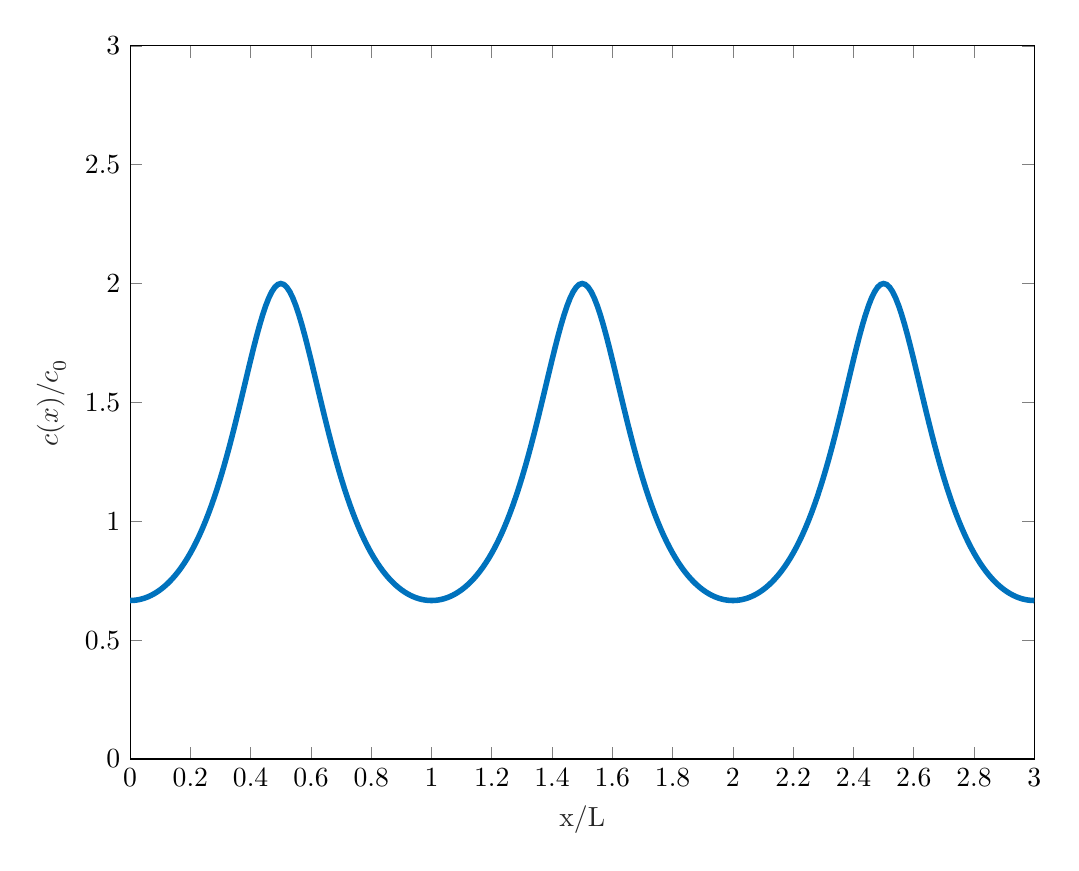
\begin{tikzpicture}

\begin{axis}[%
width=4.521in,
height=3.566in,
at={(0.758in,0.481in)},
scale only axis,
xmin=0,
xmax=3,
xlabel style={font=\color{white!15!black}},
xlabel={x/L},
ymin=0,
ymax=3,
ylabel style={font=\color{white!15!black}},
ylabel={$\text{c(x)/c}_\text{0}$},
axis background/.style={fill=white}
]
\addplot [color=mycolor1, line width=2.0pt, forget plot]
  table[row sep=crcr]{%
0	0.666666666666667\\
0.01	0.667105460079907\\
0.02	0.668423573174308\\
0.03	0.670626211311912\\
0.04	0.673722072599649\\
0.05	0.677723381086195\\
0.06	0.682645932081621\\
0.07	0.688509148350888\\
0.08	0.695336145438254\\
0.09	0.703153803774931\\
0.1	0.711992844473706\\
0.11	0.72188790478265\\
0.12	0.732877608010389\\
0.13	0.745004621294631\\
0.14	0.75831569280242\\
0.15	0.772861657754729\\
0.16	0.788697399980177\\
0.17	0.805881752436173\\
0.18	0.824477316198719\\
0.19	0.844550172723244\\
0.2	0.866169458636402\\
0.21	0.889406765875395\\
0.22	0.914335322636139\\
0.23	0.94102890239282\\
0.24	0.969560399403212\\
0.25	1\\
0.26	1.03241287024574\\
0.27	1.06685627323655\\
0.28	1.10337602502586\\
0.29	1.14200219900647\\
0.3	1.18274399763156\\
0.31	1.22558373146082\\
0.32	1.27046988346912\\
0.33	1.31730929684067\\
0.34	1.36595861277991\\
0.35	1.41621520611269\\
0.36	1.46780802315103\\
0.37	1.5203889162538\\
0.38	1.57352528281228\\
0.39	1.62669503209238\\
0.4	1.67928508681814\\
0.41	1.73059472849925\\
0.42	1.7798450560141\\
0.43	1.82619558354088\\
0.44	1.86876850828673\\
0.45	1.90668041802981\\
0.46	1.9390802288903\\
0.47	1.96519106342336\\
0.48	1.98435278558819\\
0.49	1.99606122912115\\
0.5	2\\
0.51	1.99606122912115\\
0.52	1.98435278558819\\
0.53	1.96519106342336\\
0.54	1.9390802288903\\
0.55	1.90668041802981\\
0.56	1.86876850828673\\
0.57	1.82619558354088\\
0.58	1.7798450560141\\
0.59	1.73059472849925\\
0.6	1.67928508681814\\
0.61	1.62669503209239\\
0.62	1.57352528281228\\
0.63	1.5203889162538\\
0.64	1.46780802315103\\
0.65	1.41621520611269\\
0.66	1.36595861277991\\
0.67	1.31730929684067\\
0.68	1.27046988346912\\
0.69	1.22558373146082\\
0.7	1.18274399763156\\
0.71	1.14200219900647\\
0.72	1.10337602502586\\
0.73	1.06685627323655\\
0.74	1.03241287024574\\
0.75	1\\
0.76	0.969560399403212\\
0.77	0.94102890239282\\
0.78	0.914335322636139\\
0.79	0.889406765875395\\
0.8	0.866169458636402\\
0.81	0.844550172723244\\
0.82	0.824477316198719\\
0.83	0.805881752436172\\
0.84	0.788697399980177\\
0.85	0.772861657754729\\
0.86	0.75831569280242\\
0.87	0.745004621294631\\
0.88	0.73287760801039\\
0.89	0.72188790478265\\
0.9	0.711992844473706\\
0.91	0.703153803774931\\
0.92	0.695336145438254\\
0.93	0.688509148350888\\
0.94	0.682645932081621\\
0.95	0.677723381086195\\
0.96	0.673722072599649\\
0.97	0.670626211311912\\
0.98	0.668423573174308\\
0.99	0.667105460079907\\
1	0.666666666666667\\
1.01	0.667105460079907\\
1.02	0.668423573174308\\
1.03	0.670626211311912\\
1.04	0.673722072599649\\
1.05	0.677723381086195\\
1.06	0.682645932081621\\
1.07	0.688509148350888\\
1.08	0.695336145438254\\
1.09	0.703153803774931\\
1.1	0.711992844473706\\
1.11	0.72188790478265\\
1.12	0.73287760801039\\
1.13	0.745004621294631\\
1.14	0.75831569280242\\
1.15	0.772861657754729\\
1.16	0.788697399980177\\
1.17	0.805881752436172\\
1.18	0.824477316198719\\
1.19	0.844550172723244\\
1.2	0.866169458636402\\
1.21	0.889406765875395\\
1.22	0.914335322636139\\
1.23	0.94102890239282\\
1.24	0.969560399403212\\
1.25	1\\
1.26	1.03241287024574\\
1.27	1.06685627323655\\
1.28	1.10337602502586\\
1.29	1.14200219900647\\
1.3	1.18274399763156\\
1.31	1.22558373146082\\
1.32	1.27046988346912\\
1.33	1.31730929684067\\
1.34	1.36595861277991\\
1.35	1.41621520611269\\
1.36	1.46780802315104\\
1.37	1.5203889162538\\
1.38	1.57352528281228\\
1.39	1.62669503209239\\
1.4	1.67928508681814\\
1.41	1.73059472849925\\
1.42	1.7798450560141\\
1.43	1.82619558354088\\
1.44	1.86876850828673\\
1.45	1.90668041802981\\
1.46	1.9390802288903\\
1.47	1.96519106342336\\
1.48	1.98435278558819\\
1.49	1.99606122912115\\
1.5	2\\
1.51	1.99606122912115\\
1.52	1.98435278558819\\
1.53	1.96519106342336\\
1.54	1.9390802288903\\
1.55	1.90668041802981\\
1.56	1.86876850828674\\
1.57	1.82619558354088\\
1.58	1.7798450560141\\
1.59	1.73059472849925\\
1.6	1.67928508681814\\
1.61	1.62669503209239\\
1.62	1.57352528281228\\
1.63	1.5203889162538\\
1.64	1.46780802315104\\
1.65	1.41621520611269\\
1.66	1.36595861277991\\
1.67	1.31730929684067\\
1.68	1.27046988346912\\
1.69	1.22558373146082\\
1.7	1.18274399763156\\
1.71	1.14200219900647\\
1.72	1.10337602502586\\
1.73	1.06685627323655\\
1.74	1.03241287024574\\
1.75	1\\
1.76	0.969560399403212\\
1.77	0.941028902392821\\
1.78	0.914335322636139\\
1.79	0.889406765875395\\
1.8	0.866169458636402\\
1.81	0.844550172723245\\
1.82	0.824477316198718\\
1.83	0.805881752436172\\
1.84	0.788697399980177\\
1.85	0.772861657754729\\
1.86	0.75831569280242\\
1.87	0.745004621294631\\
1.88	0.73287760801039\\
1.89	0.72188790478265\\
1.9	0.711992844473706\\
1.91	0.703153803774931\\
1.92	0.695336145438254\\
1.93	0.688509148350888\\
1.94	0.682645932081621\\
1.95	0.677723381086195\\
1.96	0.673722072599649\\
1.97	0.670626211311912\\
1.98	0.668423573174308\\
1.99	0.667105460079907\\
2	0.666666666666667\\
2.01	0.667105460079907\\
2.02	0.668423573174308\\
2.03	0.670626211311912\\
2.04	0.673722072599649\\
2.05	0.677723381086195\\
2.06	0.68264593208162\\
2.07	0.688509148350888\\
2.08	0.695336145438254\\
2.09	0.703153803774931\\
2.1	0.711992844473706\\
2.11	0.72188790478265\\
2.12	0.73287760801039\\
2.13	0.745004621294631\\
2.14	0.75831569280242\\
2.15	0.772861657754729\\
2.16	0.788697399980177\\
2.17	0.805881752436172\\
2.18	0.824477316198718\\
2.19	0.844550172723244\\
2.2	0.866169458636402\\
2.21	0.889406765875395\\
2.22	0.914335322636138\\
2.23	0.94102890239282\\
2.24	0.969560399403213\\
2.25	1\\
2.26	1.03241287024574\\
2.27	1.06685627323655\\
2.28	1.10337602502586\\
2.29	1.14200219900647\\
2.3	1.18274399763156\\
2.31	1.22558373146081\\
2.32	1.27046988346912\\
2.33	1.31730929684067\\
2.34	1.36595861277991\\
2.35	1.41621520611269\\
2.36	1.46780802315103\\
2.37	1.5203889162538\\
2.38	1.57352528281228\\
2.39	1.62669503209238\\
2.4	1.67928508681814\\
2.41	1.73059472849925\\
2.42	1.7798450560141\\
2.43	1.82619558354088\\
2.44	1.86876850828673\\
2.45	1.90668041802981\\
2.46	1.9390802288903\\
2.47	1.96519106342336\\
2.48	1.98435278558819\\
2.49	1.99606122912115\\
2.5	2\\
2.51	1.99606122912115\\
2.52	1.98435278558819\\
2.53	1.96519106342336\\
2.54	1.9390802288903\\
2.55	1.90668041802981\\
2.56	1.86876850828673\\
2.57	1.82619558354088\\
2.58	1.7798450560141\\
2.59	1.73059472849925\\
2.6	1.67928508681814\\
2.61	1.62669503209239\\
2.62	1.57352528281228\\
2.63	1.5203889162538\\
2.64	1.46780802315103\\
2.65	1.4162152061127\\
2.66	1.36595861277991\\
2.67	1.31730929684067\\
2.68	1.27046988346912\\
2.69	1.22558373146082\\
2.7	1.18274399763156\\
2.71	1.14200219900647\\
2.72	1.10337602502586\\
2.73	1.06685627323655\\
2.74	1.03241287024574\\
2.75	1\\
2.76	0.969560399403213\\
2.77	0.94102890239282\\
2.78	0.91433532263614\\
2.79	0.889406765875395\\
2.8	0.866169458636402\\
2.81	0.844550172723245\\
2.82	0.824477316198719\\
2.83	0.805881752436173\\
2.84	0.788697399980178\\
2.85	0.772861657754728\\
2.86	0.758315692802421\\
2.87	0.745004621294631\\
2.88	0.732877608010389\\
2.89	0.72188790478265\\
2.9	0.711992844473706\\
2.91	0.703153803774931\\
2.92	0.695336145438254\\
2.93	0.688509148350888\\
2.94	0.682645932081621\\
2.95	0.677723381086195\\
2.96	0.673722072599649\\
2.97	0.670626211311912\\
2.98	0.668423573174308\\
2.99	0.667105460079907\\
3	0.666666666666667\\
};
\end{axis}
\end{tikzpicture}%
		%\caption{}
	\end{solfig}
	
	Pour obtenir le réseau de caractéristiques, on intègre la relation
	$Q \mbox{d} x= P \mbox{d} t$. La courbe $\Gamma$ est définie par morceaux et vaut l'union entre l'axe $t\geqslant0$ et l'axe $x\geqslant0$.
	
	Pour la région A, on intègre d'un point $(s,0)$ sur l'axe des $x$ positifs jusque $(x,t)$. On a donc
	$$ \int_s^x \mbox{d}\overline{x}=\int_0^t c(\overline{x}) \: \mbox{d}\overline{t}$$
	$$	\int_s^x \bigg(1+\frac{1}{2}\cos(2\pi \overline{x}/L )\bigg)\mbox{d}\overline{x}=c_0 t $$
	$$	\frac{x}{L}+\frac{1}{4\pi}\sin(2\pi x/L) -\frac{s}{L}-\frac{1}{4\pi}\sin(2\pi s/L) =\frac{c_0 t}{L} $$
	Cette égalité fournit le graphe de $\frac{c_0 t}{L}$ en fonction de $x/L$ pour la région A. Le graphe ci-dessous montre la fonction pour plusieurs valeurs de $s$.
	\begin{solfig}{c}{Esquisse des caractéristiques dans la région A}
		\centering
		% This file was created by matlab2tikz.
%
%The latest updates can be retrieved from
%  http://www.mathworks.com/matlabcentral/fileexchange/22022-matlab2tikz-matlab2tikz
%where you can also make suggestions and rate matlab2tikz.
%
\definecolor{mycolor1}{rgb}{0.00000,0.44700,0.74100}%
\definecolor{mycolor2}{rgb}{0.85000,0.32500,0.09800}%
\definecolor{mycolor3}{rgb}{0.92900,0.69400,0.12500}%
\definecolor{mycolor4}{rgb}{0.49400,0.18400,0.55600}%
%
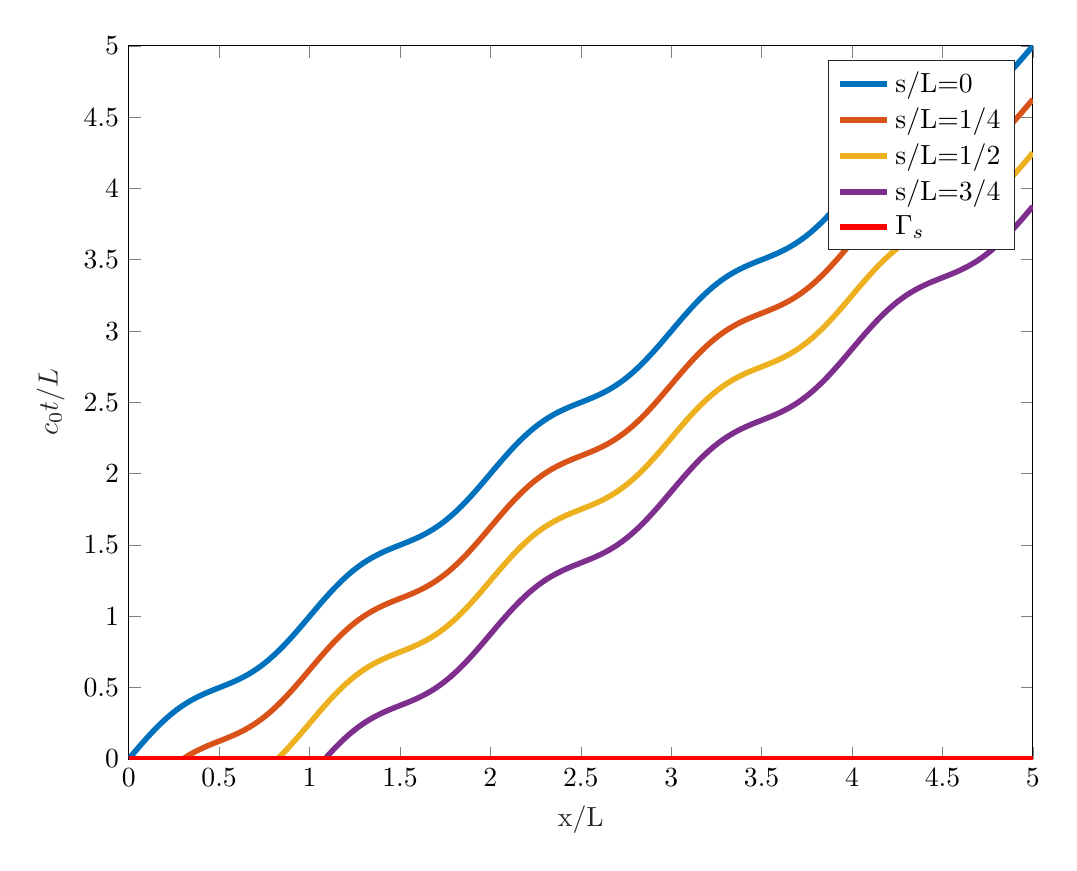
\begin{tikzpicture}

\begin{axis}[%
width=4.521in,
height=3.566in,
at={(0.758in,0.481in)},
scale only axis,
xmin=0,
xmax=5,
xlabel style={font=\color{white!15!black}},
xlabel={x/L},
ymin=0,
ymax=5,
ylabel style={font=\color{white!15!black}},
ylabel={$\text{c}_\text{0}\text{t/L}$},
axis background/.style={fill=white},
legend style={legend cell align=left, align=left, draw=white!15!black}
]
\addplot [color=mycolor1, line width=2.0pt]
  table[row sep=crcr]{%
0	0\\
0.01	0.0149967107811992\\
0.02	0.029973701827725\\
0.03	0.0449113312296878\\
0.04	0.0597901124196262\\
0.05	0.0745907910770866\\
0.06	0.0892944211166297\\
0.07	0.103882439459373\\
0.08	0.118336739292985\\
0.09	0.132639741530997\\
0.1	0.146774464189432\\
0.11	0.160724589406931\\
0.12	0.174474527843901\\
0.13	0.188009480206516\\
0.14	0.201315495652766\\
0.15	0.21437952685006\\
0.16	0.227189481467086\\
0.17	0.239734269896714\\
0.18	0.252003849021618\\
0.19	0.263989261849864\\
0.2	0.275682672864066\\
0.21	0.287077398944598\\
0.22	0.298167935744809\\
0.23	0.308949979414169\\
0.24	0.319420443583596\\
0.25	0.329577471545948\\
0.26	0.339420443583596\\
0.27	0.348949979414169\\
0.28	0.358167935744809\\
0.29	0.367077398944598\\
0.3	0.375682672864066\\
0.31	0.383989261849864\\
0.32	0.392003849021618\\
0.33	0.399734269896714\\
0.34	0.407189481467086\\
0.35	0.414379526850061\\
0.36	0.421315495652766\\
0.37	0.428009480206516\\
0.38	0.434474527843901\\
0.39	0.440724589406931\\
0.4	0.446774464189432\\
0.41	0.452639741530997\\
0.42	0.458336739292985\\
0.43	0.463882439459373\\
0.44	0.46929442111663\\
0.45	0.474590791077087\\
0.46	0.479790112419626\\
0.47	0.484911331229688\\
0.48	0.489973701827725\\
0.49	0.494996710781199\\
0.5	0.5\\
0.51	0.505003289218801\\
0.52	0.510026298172275\\
0.53	0.515088668770312\\
0.54	0.520209887580374\\
0.55	0.525409208922913\\
0.56	0.53070557888337\\
0.57	0.536117560540627\\
0.58	0.541663260707015\\
0.59	0.547360258469002\\
0.6	0.553225535810568\\
0.61	0.559275410593069\\
0.62	0.565525472156099\\
0.63	0.571990519793484\\
0.64	0.578684504347234\\
0.65	0.585620473149939\\
0.66	0.592810518532914\\
0.67	0.600265730103286\\
0.68	0.607996150978382\\
0.69	0.616010738150137\\
0.7	0.624317327135934\\
0.71	0.632922601055402\\
0.72	0.641832064255191\\
0.73	0.651050020585831\\
0.74	0.660579556416404\\
0.75	0.670422528454052\\
0.76	0.680579556416404\\
0.77	0.691050020585831\\
0.78	0.701832064255191\\
0.79	0.712922601055402\\
0.8	0.724317327135934\\
0.81	0.736010738150137\\
0.82	0.747996150978382\\
0.83	0.760265730103286\\
0.84	0.772810518532914\\
0.85	0.785620473149939\\
0.86	0.798684504347234\\
0.87	0.811990519793484\\
0.88	0.825525472156099\\
0.89	0.839275410593069\\
0.9	0.853225535810568\\
0.91	0.867360258469003\\
0.92	0.881663260707015\\
0.93	0.896117560540627\\
0.94	0.91070557888337\\
0.95	0.925409208922913\\
0.96	0.940209887580374\\
0.97	0.955088668770312\\
0.98	0.970026298172275\\
0.99	0.985003289218801\\
1	1\\
1.01	1.0149967107812\\
1.02	1.02997370182773\\
1.03	1.04491133122969\\
1.04	1.05979011241963\\
1.05	1.07459079107709\\
1.06	1.08929442111663\\
1.07	1.10388243945937\\
1.08	1.11833673929299\\
1.09	1.132639741531\\
1.1	1.14677446418943\\
1.11	1.16072458940693\\
1.12	1.1744745278439\\
1.13	1.18800948020652\\
1.14	1.20131549565277\\
1.15	1.21437952685006\\
1.16	1.22718948146709\\
1.17	1.23973426989671\\
1.18	1.25200384902162\\
1.19	1.26398926184986\\
1.2	1.27568267286407\\
1.21	1.2870773989446\\
1.22	1.29816793574481\\
1.23	1.30894997941417\\
1.24	1.3194204435836\\
1.25	1.32957747154595\\
1.26	1.3394204435836\\
1.27	1.34894997941417\\
1.28	1.35816793574481\\
1.29	1.3670773989446\\
1.3	1.37568267286407\\
1.31	1.38398926184986\\
1.32	1.39200384902162\\
1.33	1.39973426989671\\
1.34	1.40718948146709\\
1.35	1.41437952685006\\
1.36	1.42131549565277\\
1.37	1.42800948020652\\
1.38	1.4344745278439\\
1.39	1.44072458940693\\
1.4	1.44677446418943\\
1.41	1.452639741531\\
1.42	1.45833673929298\\
1.43	1.46388243945937\\
1.44	1.46929442111663\\
1.45	1.47459079107709\\
1.46	1.47979011241963\\
1.47	1.48491133122969\\
1.48	1.48997370182773\\
1.49	1.4949967107812\\
1.5	1.5\\
1.51	1.5050032892188\\
1.52	1.51002629817228\\
1.53	1.51508866877031\\
1.54	1.52020988758037\\
1.55	1.52540920892291\\
1.56	1.53070557888337\\
1.57	1.53611756054063\\
1.58	1.54166326070702\\
1.59	1.547360258469\\
1.6	1.55322553581057\\
1.61	1.55927541059307\\
1.62	1.5655254721561\\
1.63	1.57199051979348\\
1.64	1.57868450434723\\
1.65	1.58562047314994\\
1.66	1.59281051853291\\
1.67	1.60026573010329\\
1.68	1.60799615097838\\
1.69	1.61601073815014\\
1.7	1.62431732713593\\
1.71	1.6329226010554\\
1.72	1.64183206425519\\
1.73	1.65105002058583\\
1.74	1.6605795564164\\
1.75	1.67042252845405\\
1.76	1.6805795564164\\
1.77	1.69105002058583\\
1.78	1.70183206425519\\
1.79	1.7129226010554\\
1.8	1.72431732713593\\
1.81	1.73601073815014\\
1.82	1.74799615097838\\
1.83	1.76026573010329\\
1.84	1.77281051853291\\
1.85	1.78562047314994\\
1.86	1.79868450434723\\
1.87	1.81199051979348\\
1.88	1.8255254721561\\
1.89	1.83927541059307\\
1.9	1.85322553581057\\
1.91	1.867360258469\\
1.92	1.88166326070702\\
1.93	1.89611756054063\\
1.94	1.91070557888337\\
1.95	1.92540920892291\\
1.96	1.94020988758037\\
1.97	1.95508866877031\\
1.98	1.97002629817227\\
1.99	1.9850032892188\\
2	2\\
2.01	2.0149967107812\\
2.02	2.02997370182772\\
2.03	2.04491133122969\\
2.04	2.05979011241963\\
2.05	2.07459079107709\\
2.06	2.08929442111663\\
2.07	2.10388243945937\\
2.08	2.11833673929299\\
2.09	2.132639741531\\
2.1	2.14677446418943\\
2.11	2.16072458940693\\
2.12	2.1744745278439\\
2.13	2.18800948020652\\
2.14	2.20131549565277\\
2.15	2.21437952685006\\
2.16	2.22718948146709\\
2.17	2.23973426989671\\
2.18	2.25200384902162\\
2.19	2.26398926184986\\
2.2	2.27568267286407\\
2.21	2.2870773989446\\
2.22	2.29816793574481\\
2.23	2.30894997941417\\
2.24	2.3194204435836\\
2.25	2.32957747154595\\
2.26	2.3394204435836\\
2.27	2.34894997941417\\
2.28	2.35816793574481\\
2.29	2.3670773989446\\
2.3	2.37568267286407\\
2.31	2.38398926184986\\
2.32	2.39200384902162\\
2.33	2.39973426989671\\
2.34	2.40718948146709\\
2.35	2.41437952685006\\
2.36	2.42131549565277\\
2.37	2.42800948020652\\
2.38	2.4344745278439\\
2.39	2.44072458940693\\
2.4	2.44677446418943\\
2.41	2.452639741531\\
2.42	2.45833673929299\\
2.43	2.46388243945937\\
2.44	2.46929442111663\\
2.45	2.47459079107709\\
2.46	2.47979011241963\\
2.47	2.48491133122969\\
2.48	2.48997370182772\\
2.49	2.4949967107812\\
2.5	2.5\\
2.51	2.5050032892188\\
2.52	2.51002629817228\\
2.53	2.51508866877031\\
2.54	2.52020988758037\\
2.55	2.52540920892291\\
2.56	2.53070557888337\\
2.57	2.53611756054063\\
2.58	2.54166326070701\\
2.59	2.547360258469\\
2.6	2.55322553581057\\
2.61	2.55927541059307\\
2.62	2.5655254721561\\
2.63	2.57199051979348\\
2.64	2.57868450434723\\
2.65	2.58562047314994\\
2.66	2.59281051853291\\
2.67	2.60026573010329\\
2.68	2.60799615097838\\
2.69	2.61601073815014\\
2.7	2.62431732713593\\
2.71	2.6329226010554\\
2.72	2.64183206425519\\
2.73	2.65105002058583\\
2.74	2.6605795564164\\
2.75	2.67042252845405\\
2.76	2.6805795564164\\
2.77	2.69105002058583\\
2.78	2.70183206425519\\
2.79	2.7129226010554\\
2.8	2.72431732713593\\
2.81	2.73601073815014\\
2.82	2.74799615097838\\
2.83	2.76026573010329\\
2.84	2.77281051853291\\
2.85	2.78562047314994\\
2.86	2.79868450434723\\
2.87	2.81199051979348\\
2.88	2.8255254721561\\
2.89	2.83927541059307\\
2.9	2.85322553581057\\
2.91	2.867360258469\\
2.92	2.88166326070701\\
2.93	2.89611756054063\\
2.94	2.91070557888337\\
2.95	2.92540920892291\\
2.96	2.94020988758037\\
2.97	2.95508866877031\\
2.98	2.97002629817228\\
2.99	2.9850032892188\\
3	3\\
3.01	3.0149967107812\\
3.02	3.02997370182772\\
3.03	3.04491133122969\\
3.04	3.05979011241963\\
3.05	3.07459079107709\\
3.06	3.08929442111663\\
3.07	3.10388243945937\\
3.08	3.11833673929299\\
3.09	3.132639741531\\
3.1	3.14677446418943\\
3.11	3.16072458940693\\
3.12	3.1744745278439\\
3.13	3.18800948020652\\
3.14	3.20131549565277\\
3.15	3.21437952685006\\
3.16	3.22718948146709\\
3.17	3.23973426989671\\
3.18	3.25200384902162\\
3.19	3.26398926184986\\
3.2	3.27568267286407\\
3.21	3.2870773989446\\
3.22	3.29816793574481\\
3.23	3.30894997941417\\
3.24	3.3194204435836\\
3.25	3.32957747154595\\
3.26	3.3394204435836\\
3.27	3.34894997941417\\
3.28	3.35816793574481\\
3.29	3.3670773989446\\
3.3	3.37568267286407\\
3.31	3.38398926184986\\
3.32	3.39200384902162\\
3.33	3.39973426989671\\
3.34	3.40718948146709\\
3.35	3.41437952685006\\
3.36	3.42131549565277\\
3.37	3.42800948020652\\
3.38	3.4344745278439\\
3.39	3.44072458940693\\
3.4	3.44677446418943\\
3.41	3.452639741531\\
3.42	3.45833673929299\\
3.43	3.46388243945937\\
3.44	3.46929442111663\\
3.45	3.47459079107709\\
3.46	3.47979011241963\\
3.47	3.48491133122969\\
3.48	3.48997370182772\\
3.49	3.4949967107812\\
3.5	3.5\\
3.51	3.5050032892188\\
3.52	3.51002629817228\\
3.53	3.51508866877031\\
3.54	3.52020988758037\\
3.55	3.52540920892291\\
3.56	3.53070557888337\\
3.57	3.53611756054063\\
3.58	3.54166326070701\\
3.59	3.547360258469\\
3.6	3.55322553581057\\
3.61	3.55927541059307\\
3.62	3.5655254721561\\
3.63	3.57199051979348\\
3.64	3.57868450434723\\
3.65	3.58562047314994\\
3.66	3.59281051853291\\
3.67	3.60026573010329\\
3.68	3.60799615097838\\
3.69	3.61601073815014\\
3.7	3.62431732713593\\
3.71	3.6329226010554\\
3.72	3.64183206425519\\
3.73	3.65105002058583\\
3.74	3.6605795564164\\
3.75	3.67042252845405\\
3.76	3.6805795564164\\
3.77	3.69105002058583\\
3.78	3.70183206425519\\
3.79	3.7129226010554\\
3.8	3.72431732713593\\
3.81	3.73601073815014\\
3.82	3.74799615097838\\
3.83	3.76026573010329\\
3.84	3.77281051853291\\
3.85	3.78562047314994\\
3.86	3.79868450434723\\
3.87	3.81199051979348\\
3.88	3.8255254721561\\
3.89	3.83927541059307\\
3.9	3.85322553581057\\
3.91	3.867360258469\\
3.92	3.88166326070701\\
3.93	3.89611756054063\\
3.94	3.91070557888337\\
3.95	3.92540920892291\\
3.96	3.94020988758037\\
3.97	3.95508866877031\\
3.98	3.97002629817228\\
3.99	3.9850032892188\\
4	4\\
4.01	4.0149967107812\\
4.02	4.02997370182772\\
4.03	4.04491133122969\\
4.04	4.05979011241963\\
4.05	4.07459079107709\\
4.06	4.08929442111663\\
4.07	4.10388243945937\\
4.08	4.11833673929299\\
4.09	4.132639741531\\
4.1	4.14677446418943\\
4.11	4.16072458940693\\
4.12	4.1744745278439\\
4.13	4.18800948020652\\
4.14	4.20131549565277\\
4.15	4.21437952685006\\
4.16	4.22718948146709\\
4.17	4.23973426989671\\
4.18	4.25200384902162\\
4.19	4.26398926184986\\
4.2	4.27568267286407\\
4.21	4.2870773989446\\
4.22	4.29816793574481\\
4.23	4.30894997941417\\
4.24	4.3194204435836\\
4.25	4.32957747154595\\
4.26	4.3394204435836\\
4.27	4.34894997941417\\
4.28	4.35816793574481\\
4.29	4.3670773989446\\
4.3	4.37568267286407\\
4.31	4.38398926184986\\
4.32	4.39200384902162\\
4.33	4.39973426989671\\
4.34	4.40718948146709\\
4.35	4.41437952685006\\
4.36	4.42131549565277\\
4.37	4.42800948020652\\
4.38	4.4344745278439\\
4.39	4.44072458940693\\
4.4	4.44677446418943\\
4.41	4.452639741531\\
4.42	4.45833673929299\\
4.43	4.46388243945937\\
4.44	4.46929442111663\\
4.45	4.47459079107709\\
4.46	4.47979011241963\\
4.47	4.48491133122969\\
4.48	4.48997370182772\\
4.49	4.4949967107812\\
4.5	4.5\\
4.51	4.5050032892188\\
4.52	4.51002629817228\\
4.53	4.51508866877031\\
4.54	4.52020988758037\\
4.55	4.52540920892291\\
4.56	4.53070557888337\\
4.57	4.53611756054063\\
4.58	4.54166326070701\\
4.59	4.547360258469\\
4.6	4.55322553581057\\
4.61	4.55927541059307\\
4.62	4.5655254721561\\
4.63	4.57199051979348\\
4.64	4.57868450434723\\
4.65	4.58562047314994\\
4.66	4.59281051853291\\
4.67	4.60026573010329\\
4.68	4.60799615097838\\
4.69	4.61601073815014\\
4.7	4.62431732713593\\
4.71	4.6329226010554\\
4.72	4.64183206425519\\
4.73	4.65105002058583\\
4.74	4.6605795564164\\
4.75	4.67042252845405\\
4.76	4.6805795564164\\
4.77	4.69105002058583\\
4.78	4.70183206425519\\
4.79	4.7129226010554\\
4.8	4.72431732713593\\
4.81	4.73601073815014\\
4.82	4.74799615097838\\
4.83	4.76026573010329\\
4.84	4.77281051853291\\
4.85	4.78562047314994\\
4.86	4.79868450434723\\
4.87	4.81199051979348\\
4.88	4.8255254721561\\
4.89	4.83927541059307\\
4.9	4.85322553581057\\
4.91	4.867360258469\\
4.92	4.88166326070701\\
4.93	4.89611756054063\\
4.94	4.91070557888337\\
4.95	4.92540920892291\\
4.96	4.94020988758037\\
4.97	4.95508866877031\\
4.98	4.97002629817228\\
4.99	4.9850032892188\\
5	5\\
};
\addlegendentry{s/L=0}

\addplot [color=mycolor2, line width=2.0pt]
  table[row sep=crcr]{%
0	-0.375\\
0.01	-0.360003289218801\\
0.02	-0.345026298172275\\
0.03	-0.330088668770312\\
0.04	-0.315209887580374\\
0.05	-0.300409208922913\\
0.06	-0.28570557888337\\
0.07	-0.271117560540627\\
0.08	-0.256663260707015\\
0.09	-0.242360258469003\\
0.1	-0.228225535810568\\
0.11	-0.214275410593069\\
0.12	-0.200525472156099\\
0.13	-0.186990519793484\\
0.14	-0.173684504347234\\
0.15	-0.16062047314994\\
0.16	-0.147810518532914\\
0.17	-0.135265730103286\\
0.18	-0.122996150978382\\
0.19	-0.111010738150136\\
0.2	-0.0993173271359343\\
0.21	-0.0879226010554023\\
0.22	-0.0768320642551906\\
0.23	-0.0660500205858308\\
0.24	-0.055579556416404\\
0.25	-0.0454225284540523\\
0.26	-0.035579556416404\\
0.27	-0.0260500205858308\\
0.28	-0.0168320642551906\\
0.29	-0.00792260105540232\\
0.3	0.000682672864065696\\
0.31	0.00898926184986355\\
0.32	0.0170038490216184\\
0.33	0.0247342698967144\\
0.34	0.0321894814670856\\
0.35	0.0393795268500605\\
0.36	0.0463154956527662\\
0.37	0.0530094802065159\\
0.38	0.0594745278439011\\
0.39	0.0657245894069308\\
0.4	0.071774464189432\\
0.41	0.0776397415309975\\
0.42	0.083336739292985\\
0.43	0.0888824394593733\\
0.44	0.0942944211166297\\
0.45	0.0995907910770867\\
0.46	0.104790112419626\\
0.47	0.109911331229688\\
0.48	0.114973701827725\\
0.49	0.119996710781199\\
0.5	0.125\\
0.51	0.130003289218801\\
0.52	0.135026298172275\\
0.53	0.140088668770312\\
0.54	0.145209887580374\\
0.55	0.150409208922913\\
0.56	0.15570557888337\\
0.57	0.161117560540627\\
0.58	0.166663260707015\\
0.59	0.172360258469003\\
0.6	0.178225535810568\\
0.61	0.184275410593069\\
0.62	0.190525472156099\\
0.63	0.196990519793484\\
0.64	0.203684504347234\\
0.65	0.21062047314994\\
0.66	0.217810518532914\\
0.67	0.225265730103286\\
0.68	0.232996150978382\\
0.69	0.241010738150137\\
0.7	0.249317327135934\\
0.71	0.257922601055402\\
0.72	0.266832064255191\\
0.73	0.276050020585831\\
0.74	0.285579556416404\\
0.75	0.295422528454052\\
0.76	0.305579556416404\\
0.77	0.316050020585831\\
0.78	0.326832064255191\\
0.79	0.337922601055402\\
0.8	0.349317327135934\\
0.81	0.361010738150137\\
0.82	0.372996150978382\\
0.83	0.385265730103286\\
0.84	0.397810518532914\\
0.85	0.410620473149939\\
0.86	0.423684504347234\\
0.87	0.436990519793484\\
0.88	0.450525472156099\\
0.89	0.464275410593069\\
0.9	0.478225535810568\\
0.91	0.492360258469003\\
0.92	0.506663260707015\\
0.93	0.521117560540627\\
0.94	0.53570557888337\\
0.95	0.550409208922913\\
0.96	0.565209887580374\\
0.97	0.580088668770312\\
0.98	0.595026298172275\\
0.99	0.610003289218801\\
1	0.625\\
1.01	0.639996710781199\\
1.02	0.654973701827725\\
1.03	0.669911331229688\\
1.04	0.684790112419626\\
1.05	0.699590791077087\\
1.06	0.71429442111663\\
1.07	0.728882439459373\\
1.08	0.743336739292985\\
1.09	0.757639741530998\\
1.1	0.771774464189432\\
1.11	0.785724589406931\\
1.12	0.799474527843901\\
1.13	0.813009480206516\\
1.14	0.826315495652766\\
1.15	0.839379526850061\\
1.16	0.852189481467086\\
1.17	0.864734269896714\\
1.18	0.877003849021618\\
1.19	0.888989261849863\\
1.2	0.900682672864066\\
1.21	0.912077398944598\\
1.22	0.923167935744809\\
1.23	0.933949979414169\\
1.24	0.944420443583596\\
1.25	0.954577471545948\\
1.26	0.964420443583596\\
1.27	0.973949979414169\\
1.28	0.983167935744809\\
1.29	0.992077398944598\\
1.3	1.00068267286407\\
1.31	1.00898926184986\\
1.32	1.01700384902162\\
1.33	1.02473426989671\\
1.34	1.03218948146709\\
1.35	1.03937952685006\\
1.36	1.04631549565277\\
1.37	1.05300948020652\\
1.38	1.0594745278439\\
1.39	1.06572458940693\\
1.4	1.07177446418943\\
1.41	1.077639741531\\
1.42	1.08333673929298\\
1.43	1.08888243945937\\
1.44	1.09429442111663\\
1.45	1.09959079107709\\
1.46	1.10479011241963\\
1.47	1.10991133122969\\
1.48	1.11497370182773\\
1.49	1.1199967107812\\
1.5	1.125\\
1.51	1.1300032892188\\
1.52	1.13502629817228\\
1.53	1.14008866877031\\
1.54	1.14520988758037\\
1.55	1.15040920892291\\
1.56	1.15570557888337\\
1.57	1.16111756054063\\
1.58	1.16666326070702\\
1.59	1.172360258469\\
1.6	1.17822553581057\\
1.61	1.18427541059307\\
1.62	1.1905254721561\\
1.63	1.19699051979348\\
1.64	1.20368450434723\\
1.65	1.21062047314994\\
1.66	1.21781051853291\\
1.67	1.22526573010329\\
1.68	1.23299615097838\\
1.69	1.24101073815014\\
1.7	1.24931732713593\\
1.71	1.2579226010554\\
1.72	1.26683206425519\\
1.73	1.27605002058583\\
1.74	1.2855795564164\\
1.75	1.29542252845405\\
1.76	1.3055795564164\\
1.77	1.31605002058583\\
1.78	1.32683206425519\\
1.79	1.3379226010554\\
1.8	1.34931732713593\\
1.81	1.36101073815014\\
1.82	1.37299615097838\\
1.83	1.38526573010329\\
1.84	1.39781051853291\\
1.85	1.41062047314994\\
1.86	1.42368450434723\\
1.87	1.43699051979348\\
1.88	1.4505254721561\\
1.89	1.46427541059307\\
1.9	1.47822553581057\\
1.91	1.492360258469\\
1.92	1.50666326070702\\
1.93	1.52111756054063\\
1.94	1.53570557888337\\
1.95	1.55040920892291\\
1.96	1.56520988758037\\
1.97	1.58008866877031\\
1.98	1.59502629817227\\
1.99	1.6100032892188\\
2	1.625\\
2.01	1.6399967107812\\
2.02	1.65497370182772\\
2.03	1.66991133122969\\
2.04	1.68479011241963\\
2.05	1.69959079107709\\
2.06	1.71429442111663\\
2.07	1.72888243945937\\
2.08	1.74333673929299\\
2.09	1.757639741531\\
2.1	1.77177446418943\\
2.11	1.78572458940693\\
2.12	1.7994745278439\\
2.13	1.81300948020652\\
2.14	1.82631549565277\\
2.15	1.83937952685006\\
2.16	1.85218948146709\\
2.17	1.86473426989671\\
2.18	1.87700384902162\\
2.19	1.88898926184986\\
2.2	1.90068267286407\\
2.21	1.9120773989446\\
2.22	1.92316793574481\\
2.23	1.93394997941417\\
2.24	1.9444204435836\\
2.25	1.95457747154595\\
2.26	1.9644204435836\\
2.27	1.97394997941417\\
2.28	1.98316793574481\\
2.29	1.9920773989446\\
2.3	2.00068267286407\\
2.31	2.00898926184986\\
2.32	2.01700384902162\\
2.33	2.02473426989671\\
2.34	2.03218948146709\\
2.35	2.03937952685006\\
2.36	2.04631549565277\\
2.37	2.05300948020652\\
2.38	2.0594745278439\\
2.39	2.06572458940693\\
2.4	2.07177446418943\\
2.41	2.077639741531\\
2.42	2.08333673929299\\
2.43	2.08888243945937\\
2.44	2.09429442111663\\
2.45	2.09959079107709\\
2.46	2.10479011241963\\
2.47	2.10991133122969\\
2.48	2.11497370182772\\
2.49	2.1199967107812\\
2.5	2.125\\
2.51	2.1300032892188\\
2.52	2.13502629817228\\
2.53	2.14008866877031\\
2.54	2.14520988758037\\
2.55	2.15040920892291\\
2.56	2.15570557888337\\
2.57	2.16111756054063\\
2.58	2.16666326070701\\
2.59	2.172360258469\\
2.6	2.17822553581057\\
2.61	2.18427541059307\\
2.62	2.1905254721561\\
2.63	2.19699051979348\\
2.64	2.20368450434723\\
2.65	2.21062047314994\\
2.66	2.21781051853291\\
2.67	2.22526573010329\\
2.68	2.23299615097838\\
2.69	2.24101073815014\\
2.7	2.24931732713593\\
2.71	2.2579226010554\\
2.72	2.26683206425519\\
2.73	2.27605002058583\\
2.74	2.2855795564164\\
2.75	2.29542252845405\\
2.76	2.3055795564164\\
2.77	2.31605002058583\\
2.78	2.32683206425519\\
2.79	2.3379226010554\\
2.8	2.34931732713593\\
2.81	2.36101073815014\\
2.82	2.37299615097838\\
2.83	2.38526573010329\\
2.84	2.39781051853291\\
2.85	2.41062047314994\\
2.86	2.42368450434723\\
2.87	2.43699051979348\\
2.88	2.4505254721561\\
2.89	2.46427541059307\\
2.9	2.47822553581057\\
2.91	2.492360258469\\
2.92	2.50666326070701\\
2.93	2.52111756054063\\
2.94	2.53570557888337\\
2.95	2.55040920892291\\
2.96	2.56520988758037\\
2.97	2.58008866877031\\
2.98	2.59502629817228\\
2.99	2.6100032892188\\
3	2.625\\
3.01	2.6399967107812\\
3.02	2.65497370182772\\
3.03	2.66991133122969\\
3.04	2.68479011241963\\
3.05	2.69959079107709\\
3.06	2.71429442111663\\
3.07	2.72888243945937\\
3.08	2.74333673929299\\
3.09	2.757639741531\\
3.1	2.77177446418943\\
3.11	2.78572458940693\\
3.12	2.7994745278439\\
3.13	2.81300948020652\\
3.14	2.82631549565277\\
3.15	2.83937952685006\\
3.16	2.85218948146709\\
3.17	2.86473426989671\\
3.18	2.87700384902162\\
3.19	2.88898926184986\\
3.2	2.90068267286407\\
3.21	2.9120773989446\\
3.22	2.92316793574481\\
3.23	2.93394997941417\\
3.24	2.9444204435836\\
3.25	2.95457747154595\\
3.26	2.9644204435836\\
3.27	2.97394997941417\\
3.28	2.98316793574481\\
3.29	2.9920773989446\\
3.3	3.00068267286407\\
3.31	3.00898926184986\\
3.32	3.01700384902162\\
3.33	3.02473426989671\\
3.34	3.03218948146709\\
3.35	3.03937952685006\\
3.36	3.04631549565277\\
3.37	3.05300948020652\\
3.38	3.0594745278439\\
3.39	3.06572458940693\\
3.4	3.07177446418943\\
3.41	3.077639741531\\
3.42	3.08333673929299\\
3.43	3.08888243945937\\
3.44	3.09429442111663\\
3.45	3.09959079107709\\
3.46	3.10479011241963\\
3.47	3.10991133122969\\
3.48	3.11497370182772\\
3.49	3.1199967107812\\
3.5	3.125\\
3.51	3.1300032892188\\
3.52	3.13502629817228\\
3.53	3.14008866877031\\
3.54	3.14520988758037\\
3.55	3.15040920892291\\
3.56	3.15570557888337\\
3.57	3.16111756054063\\
3.58	3.16666326070701\\
3.59	3.172360258469\\
3.6	3.17822553581057\\
3.61	3.18427541059307\\
3.62	3.1905254721561\\
3.63	3.19699051979348\\
3.64	3.20368450434723\\
3.65	3.21062047314994\\
3.66	3.21781051853291\\
3.67	3.22526573010329\\
3.68	3.23299615097838\\
3.69	3.24101073815014\\
3.7	3.24931732713593\\
3.71	3.2579226010554\\
3.72	3.26683206425519\\
3.73	3.27605002058583\\
3.74	3.2855795564164\\
3.75	3.29542252845405\\
3.76	3.3055795564164\\
3.77	3.31605002058583\\
3.78	3.32683206425519\\
3.79	3.3379226010554\\
3.8	3.34931732713593\\
3.81	3.36101073815014\\
3.82	3.37299615097838\\
3.83	3.38526573010329\\
3.84	3.39781051853291\\
3.85	3.41062047314994\\
3.86	3.42368450434723\\
3.87	3.43699051979348\\
3.88	3.4505254721561\\
3.89	3.46427541059307\\
3.9	3.47822553581057\\
3.91	3.492360258469\\
3.92	3.50666326070701\\
3.93	3.52111756054063\\
3.94	3.53570557888337\\
3.95	3.55040920892291\\
3.96	3.56520988758037\\
3.97	3.58008866877031\\
3.98	3.59502629817228\\
3.99	3.6100032892188\\
4	3.625\\
4.01	3.6399967107812\\
4.02	3.65497370182772\\
4.03	3.66991133122969\\
4.04	3.68479011241963\\
4.05	3.69959079107709\\
4.06	3.71429442111663\\
4.07	3.72888243945937\\
4.08	3.74333673929298\\
4.09	3.757639741531\\
4.1	3.77177446418943\\
4.11	3.78572458940693\\
4.12	3.7994745278439\\
4.13	3.81300948020652\\
4.14	3.82631549565277\\
4.15	3.83937952685006\\
4.16	3.85218948146709\\
4.17	3.86473426989671\\
4.18	3.87700384902162\\
4.19	3.88898926184986\\
4.2	3.90068267286407\\
4.21	3.9120773989446\\
4.22	3.92316793574481\\
4.23	3.93394997941417\\
4.24	3.9444204435836\\
4.25	3.95457747154595\\
4.26	3.9644204435836\\
4.27	3.97394997941417\\
4.28	3.98316793574481\\
4.29	3.9920773989446\\
4.3	4.00068267286407\\
4.31	4.00898926184986\\
4.32	4.01700384902162\\
4.33	4.02473426989671\\
4.34	4.03218948146709\\
4.35	4.03937952685006\\
4.36	4.04631549565277\\
4.37	4.05300948020652\\
4.38	4.0594745278439\\
4.39	4.06572458940693\\
4.4	4.07177446418943\\
4.41	4.077639741531\\
4.42	4.08333673929299\\
4.43	4.08888243945937\\
4.44	4.09429442111663\\
4.45	4.09959079107709\\
4.46	4.10479011241963\\
4.47	4.10991133122969\\
4.48	4.11497370182772\\
4.49	4.1199967107812\\
4.5	4.125\\
4.51	4.1300032892188\\
4.52	4.13502629817228\\
4.53	4.14008866877031\\
4.54	4.14520988758037\\
4.55	4.15040920892291\\
4.56	4.15570557888337\\
4.57	4.16111756054063\\
4.58	4.16666326070701\\
4.59	4.172360258469\\
4.6	4.17822553581057\\
4.61	4.18427541059307\\
4.62	4.1905254721561\\
4.63	4.19699051979348\\
4.64	4.20368450434723\\
4.65	4.21062047314994\\
4.66	4.21781051853291\\
4.67	4.22526573010329\\
4.68	4.23299615097838\\
4.69	4.24101073815014\\
4.7	4.24931732713593\\
4.71	4.2579226010554\\
4.72	4.26683206425519\\
4.73	4.27605002058583\\
4.74	4.2855795564164\\
4.75	4.29542252845405\\
4.76	4.3055795564164\\
4.77	4.31605002058583\\
4.78	4.32683206425519\\
4.79	4.3379226010554\\
4.8	4.34931732713593\\
4.81	4.36101073815014\\
4.82	4.37299615097838\\
4.83	4.38526573010329\\
4.84	4.39781051853291\\
4.85	4.41062047314994\\
4.86	4.42368450434723\\
4.87	4.43699051979348\\
4.88	4.4505254721561\\
4.89	4.46427541059307\\
4.9	4.47822553581057\\
4.91	4.492360258469\\
4.92	4.50666326070701\\
4.93	4.52111756054063\\
4.94	4.53570557888337\\
4.95	4.55040920892291\\
4.96	4.56520988758037\\
4.97	4.58008866877031\\
4.98	4.59502629817228\\
4.99	4.6100032892188\\
5	4.625\\
};
\addlegendentry{s/L=1/4}

\addplot [color=mycolor3, line width=2.0pt]
  table[row sep=crcr]{%
0	-0.75\\
0.01	-0.735003289218801\\
0.02	-0.720026298172275\\
0.03	-0.705088668770312\\
0.04	-0.690209887580374\\
0.05	-0.675409208922913\\
0.06	-0.66070557888337\\
0.07	-0.646117560540627\\
0.08	-0.631663260707015\\
0.09	-0.617360258469003\\
0.1	-0.603225535810568\\
0.11	-0.589275410593069\\
0.12	-0.575525472156099\\
0.13	-0.561990519793484\\
0.14	-0.548684504347234\\
0.15	-0.535620473149939\\
0.16	-0.522810518532914\\
0.17	-0.510265730103286\\
0.18	-0.497996150978382\\
0.19	-0.486010738150136\\
0.2	-0.474317327135934\\
0.21	-0.462922601055402\\
0.22	-0.451832064255191\\
0.23	-0.441050020585831\\
0.24	-0.430579556416404\\
0.25	-0.420422528454052\\
0.26	-0.410579556416404\\
0.27	-0.401050020585831\\
0.28	-0.391832064255191\\
0.29	-0.382922601055402\\
0.3	-0.374317327135934\\
0.31	-0.366010738150136\\
0.32	-0.357996150978382\\
0.33	-0.350265730103286\\
0.34	-0.342810518532914\\
0.35	-0.335620473149939\\
0.36	-0.328684504347234\\
0.37	-0.321990519793484\\
0.38	-0.315525472156099\\
0.39	-0.309275410593069\\
0.4	-0.303225535810568\\
0.41	-0.297360258469003\\
0.42	-0.291663260707015\\
0.43	-0.286117560540627\\
0.44	-0.28070557888337\\
0.45	-0.275409208922913\\
0.46	-0.270209887580374\\
0.47	-0.265088668770312\\
0.48	-0.260026298172275\\
0.49	-0.255003289218801\\
0.5	-0.25\\
0.51	-0.244996710781199\\
0.52	-0.239973701827725\\
0.53	-0.234911331229688\\
0.54	-0.229790112419626\\
0.55	-0.224590791077087\\
0.56	-0.21929442111663\\
0.57	-0.213882439459373\\
0.58	-0.208336739292985\\
0.59	-0.202639741530997\\
0.6	-0.196774464189432\\
0.61	-0.190724589406931\\
0.62	-0.184474527843901\\
0.63	-0.178009480206516\\
0.64	-0.171315495652766\\
0.65	-0.16437952685006\\
0.66	-0.157189481467086\\
0.67	-0.149734269896714\\
0.68	-0.142003849021618\\
0.69	-0.133989261849864\\
0.7	-0.125682672864066\\
0.71	-0.117077398944598\\
0.72	-0.108167935744809\\
0.73	-0.0989499794141692\\
0.74	-0.0894204435835961\\
0.75	-0.0795774715459477\\
0.76	-0.0694204435835961\\
0.77	-0.0589499794141692\\
0.78	-0.0481679357448094\\
0.79	-0.0370773989445977\\
0.8	-0.0256826728640657\\
0.81	-0.0139892618498634\\
0.82	-0.00200384902161838\\
0.83	0.0102657301032856\\
0.84	0.0228105185329143\\
0.85	0.0356204731499395\\
0.86	0.0486845043472337\\
0.87	0.0619905197934841\\
0.88	0.0755254721560989\\
0.89	0.0892754105930692\\
0.9	0.103225535810568\\
0.91	0.117360258469003\\
0.92	0.131663260707015\\
0.93	0.146117560540627\\
0.94	0.16070557888337\\
0.95	0.175409208922913\\
0.96	0.190209887580374\\
0.97	0.205088668770312\\
0.98	0.220026298172275\\
0.99	0.235003289218801\\
1	0.25\\
1.01	0.264996710781199\\
1.02	0.279973701827725\\
1.03	0.294911331229688\\
1.04	0.309790112419626\\
1.05	0.324590791077087\\
1.06	0.33929442111663\\
1.07	0.353882439459373\\
1.08	0.368336739292985\\
1.09	0.382639741530998\\
1.1	0.396774464189432\\
1.11	0.410724589406931\\
1.12	0.424474527843901\\
1.13	0.438009480206516\\
1.14	0.451315495652766\\
1.15	0.464379526850061\\
1.16	0.477189481467086\\
1.17	0.489734269896714\\
1.18	0.502003849021618\\
1.19	0.513989261849863\\
1.2	0.525682672864066\\
1.21	0.537077398944598\\
1.22	0.548167935744809\\
1.23	0.558949979414169\\
1.24	0.569420443583596\\
1.25	0.579577471545948\\
1.26	0.589420443583596\\
1.27	0.598949979414169\\
1.28	0.608167935744809\\
1.29	0.617077398944598\\
1.3	0.625682672864066\\
1.31	0.633989261849864\\
1.32	0.642003849021618\\
1.33	0.649734269896714\\
1.34	0.657189481467086\\
1.35	0.664379526850061\\
1.36	0.671315495652766\\
1.37	0.678009480206516\\
1.38	0.684474527843901\\
1.39	0.690724589406931\\
1.4	0.696774464189432\\
1.41	0.702639741530997\\
1.42	0.708336739292985\\
1.43	0.713882439459373\\
1.44	0.71929442111663\\
1.45	0.724590791077087\\
1.46	0.729790112419626\\
1.47	0.734911331229688\\
1.48	0.739973701827725\\
1.49	0.744996710781199\\
1.5	0.75\\
1.51	0.755003289218801\\
1.52	0.760026298172275\\
1.53	0.765088668770312\\
1.54	0.770209887580374\\
1.55	0.775409208922913\\
1.56	0.78070557888337\\
1.57	0.786117560540627\\
1.58	0.791663260707015\\
1.59	0.797360258469003\\
1.6	0.803225535810568\\
1.61	0.809275410593069\\
1.62	0.815525472156099\\
1.63	0.821990519793484\\
1.64	0.828684504347234\\
1.65	0.83562047314994\\
1.66	0.842810518532914\\
1.67	0.850265730103286\\
1.68	0.857996150978382\\
1.69	0.866010738150137\\
1.7	0.874317327135934\\
1.71	0.882922601055402\\
1.72	0.891832064255191\\
1.73	0.901050020585831\\
1.74	0.910579556416404\\
1.75	0.920422528454052\\
1.76	0.930579556416404\\
1.77	0.941050020585831\\
1.78	0.951832064255191\\
1.79	0.962922601055402\\
1.8	0.974317327135934\\
1.81	0.986010738150136\\
1.82	0.997996150978382\\
1.83	1.01026573010329\\
1.84	1.02281051853291\\
1.85	1.03562047314994\\
1.86	1.04868450434723\\
1.87	1.06199051979348\\
1.88	1.0755254721561\\
1.89	1.08927541059307\\
1.9	1.10322553581057\\
1.91	1.117360258469\\
1.92	1.13166326070701\\
1.93	1.14611756054063\\
1.94	1.16070557888337\\
1.95	1.17540920892291\\
1.96	1.19020988758037\\
1.97	1.20508866877031\\
1.98	1.22002629817227\\
1.99	1.2350032892188\\
2	1.25\\
2.01	1.2649967107812\\
2.02	1.27997370182772\\
2.03	1.29491133122969\\
2.04	1.30979011241963\\
2.05	1.32459079107709\\
2.06	1.33929442111663\\
2.07	1.35388243945937\\
2.08	1.36833673929299\\
2.09	1.382639741531\\
2.1	1.39677446418943\\
2.11	1.41072458940693\\
2.12	1.4244745278439\\
2.13	1.43800948020652\\
2.14	1.45131549565277\\
2.15	1.46437952685006\\
2.16	1.47718948146709\\
2.17	1.48973426989671\\
2.18	1.50200384902162\\
2.19	1.51398926184986\\
2.2	1.52568267286407\\
2.21	1.5370773989446\\
2.22	1.54816793574481\\
2.23	1.55894997941417\\
2.24	1.5694204435836\\
2.25	1.57957747154595\\
2.26	1.5894204435836\\
2.27	1.59894997941417\\
2.28	1.60816793574481\\
2.29	1.6170773989446\\
2.3	1.62568267286407\\
2.31	1.63398926184986\\
2.32	1.64200384902162\\
2.33	1.64973426989671\\
2.34	1.65718948146709\\
2.35	1.66437952685006\\
2.36	1.67131549565277\\
2.37	1.67800948020652\\
2.38	1.6844745278439\\
2.39	1.69072458940693\\
2.4	1.69677446418943\\
2.41	1.702639741531\\
2.42	1.70833673929299\\
2.43	1.71388243945937\\
2.44	1.71929442111663\\
2.45	1.72459079107709\\
2.46	1.72979011241963\\
2.47	1.73491133122969\\
2.48	1.73997370182773\\
2.49	1.7449967107812\\
2.5	1.75\\
2.51	1.7550032892188\\
2.52	1.76002629817228\\
2.53	1.76508866877031\\
2.54	1.77020988758037\\
2.55	1.77540920892291\\
2.56	1.78070557888337\\
2.57	1.78611756054063\\
2.58	1.79166326070702\\
2.59	1.797360258469\\
2.6	1.80322553581057\\
2.61	1.80927541059307\\
2.62	1.8155254721561\\
2.63	1.82199051979348\\
2.64	1.82868450434723\\
2.65	1.83562047314994\\
2.66	1.84281051853291\\
2.67	1.85026573010329\\
2.68	1.85799615097838\\
2.69	1.86601073815014\\
2.7	1.87431732713593\\
2.71	1.8829226010554\\
2.72	1.89183206425519\\
2.73	1.90105002058583\\
2.74	1.9105795564164\\
2.75	1.92042252845405\\
2.76	1.9305795564164\\
2.77	1.94105002058583\\
2.78	1.95183206425519\\
2.79	1.9629226010554\\
2.8	1.97431732713593\\
2.81	1.98601073815014\\
2.82	1.99799615097838\\
2.83	2.01026573010329\\
2.84	2.02281051853291\\
2.85	2.03562047314994\\
2.86	2.04868450434723\\
2.87	2.06199051979348\\
2.88	2.0755254721561\\
2.89	2.08927541059307\\
2.9	2.10322553581057\\
2.91	2.117360258469\\
2.92	2.13166326070701\\
2.93	2.14611756054063\\
2.94	2.16070557888337\\
2.95	2.17540920892291\\
2.96	2.19020988758037\\
2.97	2.20508866877031\\
2.98	2.22002629817228\\
2.99	2.2350032892188\\
3	2.25\\
3.01	2.2649967107812\\
3.02	2.27997370182772\\
3.03	2.29491133122969\\
3.04	2.30979011241963\\
3.05	2.32459079107709\\
3.06	2.33929442111663\\
3.07	2.35388243945937\\
3.08	2.36833673929299\\
3.09	2.382639741531\\
3.1	2.39677446418943\\
3.11	2.41072458940693\\
3.12	2.4244745278439\\
3.13	2.43800948020652\\
3.14	2.45131549565277\\
3.15	2.46437952685006\\
3.16	2.47718948146709\\
3.17	2.48973426989671\\
3.18	2.50200384902162\\
3.19	2.51398926184986\\
3.2	2.52568267286407\\
3.21	2.5370773989446\\
3.22	2.54816793574481\\
3.23	2.55894997941417\\
3.24	2.5694204435836\\
3.25	2.57957747154595\\
3.26	2.5894204435836\\
3.27	2.59894997941417\\
3.28	2.60816793574481\\
3.29	2.6170773989446\\
3.3	2.62568267286407\\
3.31	2.63398926184986\\
3.32	2.64200384902162\\
3.33	2.64973426989671\\
3.34	2.65718948146709\\
3.35	2.66437952685006\\
3.36	2.67131549565277\\
3.37	2.67800948020652\\
3.38	2.6844745278439\\
3.39	2.69072458940693\\
3.4	2.69677446418943\\
3.41	2.702639741531\\
3.42	2.70833673929299\\
3.43	2.71388243945937\\
3.44	2.71929442111663\\
3.45	2.72459079107709\\
3.46	2.72979011241963\\
3.47	2.73491133122969\\
3.48	2.73997370182772\\
3.49	2.7449967107812\\
3.5	2.75\\
3.51	2.7550032892188\\
3.52	2.76002629817228\\
3.53	2.76508866877031\\
3.54	2.77020988758037\\
3.55	2.77540920892291\\
3.56	2.78070557888337\\
3.57	2.78611756054063\\
3.58	2.79166326070701\\
3.59	2.797360258469\\
3.6	2.80322553581057\\
3.61	2.80927541059307\\
3.62	2.8155254721561\\
3.63	2.82199051979348\\
3.64	2.82868450434723\\
3.65	2.83562047314994\\
3.66	2.84281051853291\\
3.67	2.85026573010329\\
3.68	2.85799615097838\\
3.69	2.86601073815014\\
3.7	2.87431732713593\\
3.71	2.8829226010554\\
3.72	2.89183206425519\\
3.73	2.90105002058583\\
3.74	2.9105795564164\\
3.75	2.92042252845405\\
3.76	2.9305795564164\\
3.77	2.94105002058583\\
3.78	2.95183206425519\\
3.79	2.9629226010554\\
3.8	2.97431732713593\\
3.81	2.98601073815014\\
3.82	2.99799615097838\\
3.83	3.01026573010329\\
3.84	3.02281051853291\\
3.85	3.03562047314994\\
3.86	3.04868450434723\\
3.87	3.06199051979348\\
3.88	3.0755254721561\\
3.89	3.08927541059307\\
3.9	3.10322553581057\\
3.91	3.117360258469\\
3.92	3.13166326070701\\
3.93	3.14611756054063\\
3.94	3.16070557888337\\
3.95	3.17540920892291\\
3.96	3.19020988758037\\
3.97	3.20508866877031\\
3.98	3.22002629817228\\
3.99	3.2350032892188\\
4	3.25\\
4.01	3.2649967107812\\
4.02	3.27997370182772\\
4.03	3.29491133122969\\
4.04	3.30979011241963\\
4.05	3.32459079107709\\
4.06	3.33929442111663\\
4.07	3.35388243945937\\
4.08	3.36833673929299\\
4.09	3.382639741531\\
4.1	3.39677446418943\\
4.11	3.41072458940693\\
4.12	3.4244745278439\\
4.13	3.43800948020652\\
4.14	3.45131549565277\\
4.15	3.46437952685006\\
4.16	3.47718948146709\\
4.17	3.48973426989671\\
4.18	3.50200384902162\\
4.19	3.51398926184986\\
4.2	3.52568267286407\\
4.21	3.5370773989446\\
4.22	3.54816793574481\\
4.23	3.55894997941417\\
4.24	3.5694204435836\\
4.25	3.57957747154595\\
4.26	3.5894204435836\\
4.27	3.59894997941417\\
4.28	3.60816793574481\\
4.29	3.6170773989446\\
4.3	3.62568267286407\\
4.31	3.63398926184986\\
4.32	3.64200384902162\\
4.33	3.64973426989671\\
4.34	3.65718948146709\\
4.35	3.66437952685006\\
4.36	3.67131549565277\\
4.37	3.67800948020652\\
4.38	3.6844745278439\\
4.39	3.69072458940693\\
4.4	3.69677446418943\\
4.41	3.702639741531\\
4.42	3.70833673929299\\
4.43	3.71388243945937\\
4.44	3.71929442111663\\
4.45	3.72459079107709\\
4.46	3.72979011241963\\
4.47	3.73491133122969\\
4.48	3.73997370182773\\
4.49	3.7449967107812\\
4.5	3.75\\
4.51	3.7550032892188\\
4.52	3.76002629817228\\
4.53	3.76508866877031\\
4.54	3.77020988758037\\
4.55	3.77540920892291\\
4.56	3.78070557888337\\
4.57	3.78611756054063\\
4.58	3.79166326070701\\
4.59	3.797360258469\\
4.6	3.80322553581057\\
4.61	3.80927541059307\\
4.62	3.8155254721561\\
4.63	3.82199051979348\\
4.64	3.82868450434723\\
4.65	3.83562047314994\\
4.66	3.84281051853291\\
4.67	3.85026573010329\\
4.68	3.85799615097838\\
4.69	3.86601073815014\\
4.7	3.87431732713593\\
4.71	3.8829226010554\\
4.72	3.89183206425519\\
4.73	3.90105002058583\\
4.74	3.9105795564164\\
4.75	3.92042252845405\\
4.76	3.9305795564164\\
4.77	3.94105002058583\\
4.78	3.95183206425519\\
4.79	3.9629226010554\\
4.8	3.97431732713593\\
4.81	3.98601073815014\\
4.82	3.99799615097838\\
4.83	4.01026573010329\\
4.84	4.02281051853291\\
4.85	4.03562047314994\\
4.86	4.04868450434723\\
4.87	4.06199051979348\\
4.88	4.0755254721561\\
4.89	4.08927541059307\\
4.9	4.10322553581057\\
4.91	4.117360258469\\
4.92	4.13166326070701\\
4.93	4.14611756054063\\
4.94	4.16070557888337\\
4.95	4.17540920892291\\
4.96	4.19020988758037\\
4.97	4.20508866877031\\
4.98	4.22002629817228\\
4.99	4.2350032892188\\
5	4.25\\
};
\addlegendentry{s/L=1/2}

\addplot [color=mycolor4, line width=2.0pt]
  table[row sep=crcr]{%
0	-1.125\\
0.01	-1.1100032892188\\
0.02	-1.09502629817227\\
0.03	-1.08008866877031\\
0.04	-1.06520988758037\\
0.05	-1.05040920892291\\
0.06	-1.03570557888337\\
0.07	-1.02111756054063\\
0.08	-1.00666326070702\\
0.09	-0.992360258469003\\
0.1	-0.978225535810568\\
0.11	-0.964275410593069\\
0.12	-0.950525472156099\\
0.13	-0.936990519793484\\
0.14	-0.923684504347234\\
0.15	-0.910620473149939\\
0.16	-0.897810518532914\\
0.17	-0.885265730103286\\
0.18	-0.872996150978382\\
0.19	-0.861010738150137\\
0.2	-0.849317327135934\\
0.21	-0.837922601055402\\
0.22	-0.826832064255191\\
0.23	-0.816050020585831\\
0.24	-0.805579556416404\\
0.25	-0.795422528454052\\
0.26	-0.785579556416404\\
0.27	-0.776050020585831\\
0.28	-0.766832064255191\\
0.29	-0.757922601055402\\
0.3	-0.749317327135934\\
0.31	-0.741010738150137\\
0.32	-0.732996150978382\\
0.33	-0.725265730103286\\
0.34	-0.717810518532914\\
0.35	-0.710620473149939\\
0.36	-0.703684504347234\\
0.37	-0.696990519793484\\
0.38	-0.690525472156099\\
0.39	-0.684275410593069\\
0.4	-0.678225535810568\\
0.41	-0.672360258469002\\
0.42	-0.666663260707015\\
0.43	-0.661117560540627\\
0.44	-0.65570557888337\\
0.45	-0.650409208922913\\
0.46	-0.645209887580374\\
0.47	-0.640088668770312\\
0.48	-0.635026298172275\\
0.49	-0.630003289218801\\
0.5	-0.625\\
0.51	-0.619996710781199\\
0.52	-0.614973701827725\\
0.53	-0.609911331229688\\
0.54	-0.604790112419626\\
0.55	-0.599590791077087\\
0.56	-0.59429442111663\\
0.57	-0.588882439459373\\
0.58	-0.583336739292985\\
0.59	-0.577639741530998\\
0.6	-0.571774464189432\\
0.61	-0.565724589406931\\
0.62	-0.559474527843901\\
0.63	-0.553009480206516\\
0.64	-0.546315495652766\\
0.65	-0.539379526850061\\
0.66	-0.532189481467086\\
0.67	-0.524734269896714\\
0.68	-0.517003849021618\\
0.69	-0.508989261849863\\
0.7	-0.500682672864066\\
0.71	-0.492077398944598\\
0.72	-0.483167935744809\\
0.73	-0.473949979414169\\
0.74	-0.464420443583596\\
0.75	-0.454577471545948\\
0.76	-0.444420443583596\\
0.77	-0.433949979414169\\
0.78	-0.423167935744809\\
0.79	-0.412077398944598\\
0.8	-0.400682672864066\\
0.81	-0.388989261849863\\
0.82	-0.377003849021618\\
0.83	-0.364734269896714\\
0.84	-0.352189481467086\\
0.85	-0.339379526850061\\
0.86	-0.326315495652766\\
0.87	-0.313009480206516\\
0.88	-0.299474527843901\\
0.89	-0.285724589406931\\
0.9	-0.271774464189432\\
0.91	-0.257639741530997\\
0.92	-0.243336739292985\\
0.93	-0.228882439459373\\
0.94	-0.21429442111663\\
0.95	-0.199590791077087\\
0.96	-0.184790112419626\\
0.97	-0.169911331229688\\
0.98	-0.154973701827725\\
0.99	-0.139996710781199\\
1	-0.125\\
1.01	-0.110003289218801\\
1.02	-0.095026298172275\\
1.03	-0.0800886687703123\\
1.04	-0.0652098875803738\\
1.05	-0.0504092089229133\\
1.06	-0.0357055788833702\\
1.07	-0.0211175605406266\\
1.08	-0.0066632607070149\\
1.09	0.0076397415309975\\
1.1	0.0217744641894321\\
1.11	0.0357245894069309\\
1.12	0.0494745278439012\\
1.13	0.063009480206516\\
1.14	0.0763154956527664\\
1.15	0.0893795268500607\\
1.16	0.102189481467086\\
1.17	0.114734269896714\\
1.18	0.127003849021618\\
1.19	0.138989261849863\\
1.2	0.150682672864066\\
1.21	0.162077398944598\\
1.22	0.173167935744809\\
1.23	0.183949979414169\\
1.24	0.194420443583596\\
1.25	0.204577471545948\\
1.26	0.214420443583596\\
1.27	0.223949979414169\\
1.28	0.233167935744809\\
1.29	0.242077398944598\\
1.3	0.250682672864066\\
1.31	0.258989261849864\\
1.32	0.267003849021618\\
1.33	0.274734269896714\\
1.34	0.282189481467086\\
1.35	0.289379526850061\\
1.36	0.296315495652766\\
1.37	0.303009480206516\\
1.38	0.309474527843901\\
1.39	0.315724589406931\\
1.4	0.321774464189432\\
1.41	0.327639741530997\\
1.42	0.333336739292985\\
1.43	0.338882439459373\\
1.44	0.34429442111663\\
1.45	0.349590791077087\\
1.46	0.354790112419626\\
1.47	0.359911331229688\\
1.48	0.364973701827725\\
1.49	0.369996710781199\\
1.5	0.375\\
1.51	0.380003289218801\\
1.52	0.385026298172275\\
1.53	0.390088668770312\\
1.54	0.395209887580374\\
1.55	0.400409208922913\\
1.56	0.40570557888337\\
1.57	0.411117560540627\\
1.58	0.416663260707015\\
1.59	0.422360258469003\\
1.6	0.428225535810568\\
1.61	0.434275410593069\\
1.62	0.440525472156099\\
1.63	0.446990519793484\\
1.64	0.453684504347234\\
1.65	0.46062047314994\\
1.66	0.467810518532915\\
1.67	0.475265730103286\\
1.68	0.482996150978382\\
1.69	0.491010738150136\\
1.7	0.499317327135934\\
1.71	0.507922601055402\\
1.72	0.516832064255191\\
1.73	0.526050020585831\\
1.74	0.535579556416404\\
1.75	0.545422528454052\\
1.76	0.555579556416404\\
1.77	0.566050020585831\\
1.78	0.576832064255191\\
1.79	0.587922601055402\\
1.8	0.599317327135934\\
1.81	0.611010738150136\\
1.82	0.622996150978382\\
1.83	0.635265730103286\\
1.84	0.647810518532914\\
1.85	0.66062047314994\\
1.86	0.673684504347234\\
1.87	0.686990519793484\\
1.88	0.700525472156099\\
1.89	0.714275410593069\\
1.9	0.728225535810568\\
1.91	0.742360258469003\\
1.92	0.756663260707015\\
1.93	0.771117560540627\\
1.94	0.78570557888337\\
1.95	0.800409208922913\\
1.96	0.815209887580374\\
1.97	0.830088668770312\\
1.98	0.845026298172275\\
1.99	0.860003289218801\\
2	0.875\\
2.01	0.889996710781199\\
2.02	0.904973701827725\\
2.03	0.919911331229688\\
2.04	0.934790112419626\\
2.05	0.949590791077086\\
2.06	0.96429442111663\\
2.07	0.978882439459373\\
2.08	0.993336739292985\\
2.09	1.007639741531\\
2.1	1.02177446418943\\
2.11	1.03572458940693\\
2.12	1.0494745278439\\
2.13	1.06300948020652\\
2.14	1.07631549565277\\
2.15	1.08937952685006\\
2.16	1.10218948146709\\
2.17	1.11473426989671\\
2.18	1.12700384902162\\
2.19	1.13898926184986\\
2.2	1.15068267286407\\
2.21	1.1620773989446\\
2.22	1.17316793574481\\
2.23	1.18394997941417\\
2.24	1.1944204435836\\
2.25	1.20457747154595\\
2.26	1.2144204435836\\
2.27	1.22394997941417\\
2.28	1.23316793574481\\
2.29	1.2420773989446\\
2.3	1.25068267286407\\
2.31	1.25898926184986\\
2.32	1.26700384902162\\
2.33	1.27473426989671\\
2.34	1.28218948146709\\
2.35	1.28937952685006\\
2.36	1.29631549565277\\
2.37	1.30300948020652\\
2.38	1.3094745278439\\
2.39	1.31572458940693\\
2.4	1.32177446418943\\
2.41	1.327639741531\\
2.42	1.33333673929298\\
2.43	1.33888243945937\\
2.44	1.34429442111663\\
2.45	1.34959079107709\\
2.46	1.35479011241963\\
2.47	1.35991133122969\\
2.48	1.36497370182773\\
2.49	1.3699967107812\\
2.5	1.375\\
2.51	1.3800032892188\\
2.52	1.38502629817228\\
2.53	1.39008866877031\\
2.54	1.39520988758037\\
2.55	1.40040920892291\\
2.56	1.40570557888337\\
2.57	1.41111756054063\\
2.58	1.41666326070702\\
2.59	1.422360258469\\
2.6	1.42822553581057\\
2.61	1.43427541059307\\
2.62	1.4405254721561\\
2.63	1.44699051979348\\
2.64	1.45368450434723\\
2.65	1.46062047314994\\
2.66	1.46781051853291\\
2.67	1.47526573010329\\
2.68	1.48299615097838\\
2.69	1.49101073815014\\
2.7	1.49931732713593\\
2.71	1.5079226010554\\
2.72	1.51683206425519\\
2.73	1.52605002058583\\
2.74	1.5355795564164\\
2.75	1.54542252845405\\
2.76	1.5555795564164\\
2.77	1.56605002058583\\
2.78	1.57683206425519\\
2.79	1.5879226010554\\
2.8	1.59931732713593\\
2.81	1.61101073815014\\
2.82	1.62299615097838\\
2.83	1.63526573010329\\
2.84	1.64781051853291\\
2.85	1.66062047314994\\
2.86	1.67368450434723\\
2.87	1.68699051979348\\
2.88	1.7005254721561\\
2.89	1.71427541059307\\
2.9	1.72822553581057\\
2.91	1.742360258469\\
2.92	1.75666326070701\\
2.93	1.77111756054063\\
2.94	1.78570557888337\\
2.95	1.80040920892291\\
2.96	1.81520988758037\\
2.97	1.83008866877031\\
2.98	1.84502629817227\\
2.99	1.8600032892188\\
3	1.875\\
3.01	1.8899967107812\\
3.02	1.90497370182772\\
3.03	1.91991133122969\\
3.04	1.93479011241963\\
3.05	1.94959079107709\\
3.06	1.96429442111663\\
3.07	1.97888243945937\\
3.08	1.99333673929299\\
3.09	2.007639741531\\
3.1	2.02177446418943\\
3.11	2.03572458940693\\
3.12	2.0494745278439\\
3.13	2.06300948020652\\
3.14	2.07631549565277\\
3.15	2.08937952685006\\
3.16	2.10218948146709\\
3.17	2.11473426989671\\
3.18	2.12700384902162\\
3.19	2.13898926184986\\
3.2	2.15068267286407\\
3.21	2.1620773989446\\
3.22	2.17316793574481\\
3.23	2.18394997941417\\
3.24	2.1944204435836\\
3.25	2.20457747154595\\
3.26	2.2144204435836\\
3.27	2.22394997941417\\
3.28	2.23316793574481\\
3.29	2.2420773989446\\
3.3	2.25068267286407\\
3.31	2.25898926184986\\
3.32	2.26700384902162\\
3.33	2.27473426989671\\
3.34	2.28218948146709\\
3.35	2.28937952685006\\
3.36	2.29631549565277\\
3.37	2.30300948020652\\
3.38	2.3094745278439\\
3.39	2.31572458940693\\
3.4	2.32177446418943\\
3.41	2.327639741531\\
3.42	2.33333673929299\\
3.43	2.33888243945937\\
3.44	2.34429442111663\\
3.45	2.34959079107709\\
3.46	2.35479011241963\\
3.47	2.35991133122969\\
3.48	2.36497370182772\\
3.49	2.3699967107812\\
3.5	2.375\\
3.51	2.3800032892188\\
3.52	2.38502629817228\\
3.53	2.39008866877031\\
3.54	2.39520988758037\\
3.55	2.40040920892291\\
3.56	2.40570557888337\\
3.57	2.41111756054063\\
3.58	2.41666326070701\\
3.59	2.422360258469\\
3.6	2.42822553581057\\
3.61	2.43427541059307\\
3.62	2.4405254721561\\
3.63	2.44699051979348\\
3.64	2.45368450434723\\
3.65	2.46062047314994\\
3.66	2.46781051853291\\
3.67	2.47526573010329\\
3.68	2.48299615097838\\
3.69	2.49101073815014\\
3.7	2.49931732713593\\
3.71	2.5079226010554\\
3.72	2.51683206425519\\
3.73	2.52605002058583\\
3.74	2.5355795564164\\
3.75	2.54542252845405\\
3.76	2.5555795564164\\
3.77	2.56605002058583\\
3.78	2.57683206425519\\
3.79	2.5879226010554\\
3.8	2.59931732713593\\
3.81	2.61101073815014\\
3.82	2.62299615097838\\
3.83	2.63526573010329\\
3.84	2.64781051853291\\
3.85	2.66062047314994\\
3.86	2.67368450434723\\
3.87	2.68699051979348\\
3.88	2.7005254721561\\
3.89	2.71427541059307\\
3.9	2.72822553581057\\
3.91	2.742360258469\\
3.92	2.75666326070701\\
3.93	2.77111756054063\\
3.94	2.78570557888337\\
3.95	2.80040920892291\\
3.96	2.81520988758037\\
3.97	2.83008866877031\\
3.98	2.84502629817228\\
3.99	2.8600032892188\\
4	2.875\\
4.01	2.8899967107812\\
4.02	2.90497370182772\\
4.03	2.91991133122969\\
4.04	2.93479011241963\\
4.05	2.94959079107709\\
4.06	2.96429442111663\\
4.07	2.97888243945937\\
4.08	2.99333673929299\\
4.09	3.007639741531\\
4.1	3.02177446418943\\
4.11	3.03572458940693\\
4.12	3.0494745278439\\
4.13	3.06300948020652\\
4.14	3.07631549565277\\
4.15	3.08937952685006\\
4.16	3.10218948146709\\
4.17	3.11473426989671\\
4.18	3.12700384902162\\
4.19	3.13898926184986\\
4.2	3.15068267286407\\
4.21	3.1620773989446\\
4.22	3.17316793574481\\
4.23	3.18394997941417\\
4.24	3.1944204435836\\
4.25	3.20457747154595\\
4.26	3.2144204435836\\
4.27	3.22394997941417\\
4.28	3.23316793574481\\
4.29	3.2420773989446\\
4.3	3.25068267286407\\
4.31	3.25898926184986\\
4.32	3.26700384902162\\
4.33	3.27473426989671\\
4.34	3.28218948146709\\
4.35	3.28937952685006\\
4.36	3.29631549565277\\
4.37	3.30300948020652\\
4.38	3.3094745278439\\
4.39	3.31572458940693\\
4.4	3.32177446418943\\
4.41	3.327639741531\\
4.42	3.33333673929299\\
4.43	3.33888243945937\\
4.44	3.34429442111663\\
4.45	3.34959079107709\\
4.46	3.35479011241963\\
4.47	3.35991133122969\\
4.48	3.36497370182773\\
4.49	3.3699967107812\\
4.5	3.375\\
4.51	3.3800032892188\\
4.52	3.38502629817228\\
4.53	3.39008866877031\\
4.54	3.39520988758037\\
4.55	3.40040920892291\\
4.56	3.40570557888337\\
4.57	3.41111756054063\\
4.58	3.41666326070701\\
4.59	3.422360258469\\
4.6	3.42822553581057\\
4.61	3.43427541059307\\
4.62	3.4405254721561\\
4.63	3.44699051979348\\
4.64	3.45368450434723\\
4.65	3.46062047314994\\
4.66	3.46781051853291\\
4.67	3.47526573010329\\
4.68	3.48299615097838\\
4.69	3.49101073815014\\
4.7	3.49931732713593\\
4.71	3.5079226010554\\
4.72	3.51683206425519\\
4.73	3.52605002058583\\
4.74	3.5355795564164\\
4.75	3.54542252845405\\
4.76	3.5555795564164\\
4.77	3.56605002058583\\
4.78	3.57683206425519\\
4.79	3.5879226010554\\
4.8	3.59931732713593\\
4.81	3.61101073815014\\
4.82	3.62299615097838\\
4.83	3.63526573010329\\
4.84	3.64781051853291\\
4.85	3.66062047314994\\
4.86	3.67368450434723\\
4.87	3.68699051979348\\
4.88	3.7005254721561\\
4.89	3.71427541059307\\
4.9	3.72822553581057\\
4.91	3.742360258469\\
4.92	3.75666326070701\\
4.93	3.77111756054063\\
4.94	3.78570557888337\\
4.95	3.80040920892291\\
4.96	3.81520988758037\\
4.97	3.83008866877031\\
4.98	3.84502629817228\\
4.99	3.8600032892188\\
5	3.875\\
};
\addlegendentry{s/L=3/4}

\addplot [color=red, line width=2.0pt]
  table[row sep=crcr]{%
0	0\\
0.01	0\\
0.02	0\\
0.03	0\\
0.04	0\\
0.05	0\\
0.06	0\\
0.07	0\\
0.08	0\\
0.09	0\\
0.1	0\\
0.11	0\\
0.12	0\\
0.13	0\\
0.14	0\\
0.15	0\\
0.16	0\\
0.17	0\\
0.18	0\\
0.19	0\\
0.2	0\\
0.21	0\\
0.22	0\\
0.23	0\\
0.24	0\\
0.25	0\\
0.26	0\\
0.27	0\\
0.28	0\\
0.29	0\\
0.3	0\\
0.31	0\\
0.32	0\\
0.33	0\\
0.34	0\\
0.35	0\\
0.36	0\\
0.37	0\\
0.38	0\\
0.39	0\\
0.4	0\\
0.41	0\\
0.42	0\\
0.43	0\\
0.44	0\\
0.45	0\\
0.46	0\\
0.47	0\\
0.48	0\\
0.49	0\\
0.5	0\\
0.51	0\\
0.52	0\\
0.53	0\\
0.54	0\\
0.55	0\\
0.56	0\\
0.57	0\\
0.58	0\\
0.59	0\\
0.6	0\\
0.61	0\\
0.62	0\\
0.63	0\\
0.64	0\\
0.65	0\\
0.66	0\\
0.67	0\\
0.68	0\\
0.69	0\\
0.7	0\\
0.71	0\\
0.72	0\\
0.73	0\\
0.74	0\\
0.75	0\\
0.76	0\\
0.77	0\\
0.78	0\\
0.79	0\\
0.8	0\\
0.81	0\\
0.82	0\\
0.83	0\\
0.84	0\\
0.85	0\\
0.86	0\\
0.87	0\\
0.88	0\\
0.89	0\\
0.9	0\\
0.91	0\\
0.92	0\\
0.93	0\\
0.94	0\\
0.95	0\\
0.96	0\\
0.97	0\\
0.98	0\\
0.99	0\\
1	0\\
1.01	0\\
1.02	0\\
1.03	0\\
1.04	0\\
1.05	0\\
1.06	0\\
1.07	0\\
1.08	0\\
1.09	0\\
1.1	0\\
1.11	0\\
1.12	0\\
1.13	0\\
1.14	0\\
1.15	0\\
1.16	0\\
1.17	0\\
1.18	0\\
1.19	0\\
1.2	0\\
1.21	0\\
1.22	0\\
1.23	0\\
1.24	0\\
1.25	0\\
1.26	0\\
1.27	0\\
1.28	0\\
1.29	0\\
1.3	0\\
1.31	0\\
1.32	0\\
1.33	0\\
1.34	0\\
1.35	0\\
1.36	0\\
1.37	0\\
1.38	0\\
1.39	0\\
1.4	0\\
1.41	0\\
1.42	0\\
1.43	0\\
1.44	0\\
1.45	0\\
1.46	0\\
1.47	0\\
1.48	0\\
1.49	0\\
1.5	0\\
1.51	0\\
1.52	0\\
1.53	0\\
1.54	0\\
1.55	0\\
1.56	0\\
1.57	0\\
1.58	0\\
1.59	0\\
1.6	0\\
1.61	0\\
1.62	0\\
1.63	0\\
1.64	0\\
1.65	0\\
1.66	0\\
1.67	0\\
1.68	0\\
1.69	0\\
1.7	0\\
1.71	0\\
1.72	0\\
1.73	0\\
1.74	0\\
1.75	0\\
1.76	0\\
1.77	0\\
1.78	0\\
1.79	0\\
1.8	0\\
1.81	0\\
1.82	0\\
1.83	0\\
1.84	0\\
1.85	0\\
1.86	0\\
1.87	0\\
1.88	0\\
1.89	0\\
1.9	0\\
1.91	0\\
1.92	0\\
1.93	0\\
1.94	0\\
1.95	0\\
1.96	0\\
1.97	0\\
1.98	0\\
1.99	0\\
2	0\\
2.01	0\\
2.02	0\\
2.03	0\\
2.04	0\\
2.05	0\\
2.06	0\\
2.07	0\\
2.08	0\\
2.09	0\\
2.1	0\\
2.11	0\\
2.12	0\\
2.13	0\\
2.14	0\\
2.15	0\\
2.16	0\\
2.17	0\\
2.18	0\\
2.19	0\\
2.2	0\\
2.21	0\\
2.22	0\\
2.23	0\\
2.24	0\\
2.25	0\\
2.26	0\\
2.27	0\\
2.28	0\\
2.29	0\\
2.3	0\\
2.31	0\\
2.32	0\\
2.33	0\\
2.34	0\\
2.35	0\\
2.36	0\\
2.37	0\\
2.38	0\\
2.39	0\\
2.4	0\\
2.41	0\\
2.42	0\\
2.43	0\\
2.44	0\\
2.45	0\\
2.46	0\\
2.47	0\\
2.48	0\\
2.49	0\\
2.5	0\\
2.51	0\\
2.52	0\\
2.53	0\\
2.54	0\\
2.55	0\\
2.56	0\\
2.57	0\\
2.58	0\\
2.59	0\\
2.6	0\\
2.61	0\\
2.62	0\\
2.63	0\\
2.64	0\\
2.65	0\\
2.66	0\\
2.67	0\\
2.68	0\\
2.69	0\\
2.7	0\\
2.71	0\\
2.72	0\\
2.73	0\\
2.74	0\\
2.75	0\\
2.76	0\\
2.77	0\\
2.78	0\\
2.79	0\\
2.8	0\\
2.81	0\\
2.82	0\\
2.83	0\\
2.84	0\\
2.85	0\\
2.86	0\\
2.87	0\\
2.88	0\\
2.89	0\\
2.9	0\\
2.91	0\\
2.92	0\\
2.93	0\\
2.94	0\\
2.95	0\\
2.96	0\\
2.97	0\\
2.98	0\\
2.99	0\\
3	0\\
3.01	0\\
3.02	0\\
3.03	0\\
3.04	0\\
3.05	0\\
3.06	0\\
3.07	0\\
3.08	0\\
3.09	0\\
3.1	0\\
3.11	0\\
3.12	0\\
3.13	0\\
3.14	0\\
3.15	0\\
3.16	0\\
3.17	0\\
3.18	0\\
3.19	0\\
3.2	0\\
3.21	0\\
3.22	0\\
3.23	0\\
3.24	0\\
3.25	0\\
3.26	0\\
3.27	0\\
3.28	0\\
3.29	0\\
3.3	0\\
3.31	0\\
3.32	0\\
3.33	0\\
3.34	0\\
3.35	0\\
3.36	0\\
3.37	0\\
3.38	0\\
3.39	0\\
3.4	0\\
3.41	0\\
3.42	0\\
3.43	0\\
3.44	0\\
3.45	0\\
3.46	0\\
3.47	0\\
3.48	0\\
3.49	0\\
3.5	0\\
3.51	0\\
3.52	0\\
3.53	0\\
3.54	0\\
3.55	0\\
3.56	0\\
3.57	0\\
3.58	0\\
3.59	0\\
3.6	0\\
3.61	0\\
3.62	0\\
3.63	0\\
3.64	0\\
3.65	0\\
3.66	0\\
3.67	0\\
3.68	0\\
3.69	0\\
3.7	0\\
3.71	0\\
3.72	0\\
3.73	0\\
3.74	0\\
3.75	0\\
3.76	0\\
3.77	0\\
3.78	0\\
3.79	0\\
3.8	0\\
3.81	0\\
3.82	0\\
3.83	0\\
3.84	0\\
3.85	0\\
3.86	0\\
3.87	0\\
3.88	0\\
3.89	0\\
3.9	0\\
3.91	0\\
3.92	0\\
3.93	0\\
3.94	0\\
3.95	0\\
3.96	0\\
3.97	0\\
3.98	0\\
3.99	0\\
4	0\\
4.01	0\\
4.02	0\\
4.03	0\\
4.04	0\\
4.05	0\\
4.06	0\\
4.07	0\\
4.08	0\\
4.09	0\\
4.1	0\\
4.11	0\\
4.12	0\\
4.13	0\\
4.14	0\\
4.15	0\\
4.16	0\\
4.17	0\\
4.18	0\\
4.19	0\\
4.2	0\\
4.21	0\\
4.22	0\\
4.23	0\\
4.24	0\\
4.25	0\\
4.26	0\\
4.27	0\\
4.28	0\\
4.29	0\\
4.3	0\\
4.31	0\\
4.32	0\\
4.33	0\\
4.34	0\\
4.35	0\\
4.36	0\\
4.37	0\\
4.38	0\\
4.39	0\\
4.4	0\\
4.41	0\\
4.42	0\\
4.43	0\\
4.44	0\\
4.45	0\\
4.46	0\\
4.47	0\\
4.48	0\\
4.49	0\\
4.5	0\\
4.51	0\\
4.52	0\\
4.53	0\\
4.54	0\\
4.55	0\\
4.56	0\\
4.57	0\\
4.58	0\\
4.59	0\\
4.6	0\\
4.61	0\\
4.62	0\\
4.63	0\\
4.64	0\\
4.65	0\\
4.66	0\\
4.67	0\\
4.68	0\\
4.69	0\\
4.7	0\\
4.71	0\\
4.72	0\\
4.73	0\\
4.74	0\\
4.75	0\\
4.76	0\\
4.77	0\\
4.78	0\\
4.79	0\\
4.8	0\\
4.81	0\\
4.82	0\\
4.83	0\\
4.84	0\\
4.85	0\\
4.86	0\\
4.87	0\\
4.88	0\\
4.89	0\\
4.9	0\\
4.91	0\\
4.92	0\\
4.93	0\\
4.94	0\\
4.95	0\\
4.96	0\\
4.97	0\\
4.98	0\\
4.99	0\\
5	0\\
};
\addlegendentry{$\Gamma{}_\text{s}$}

\end{axis}
\end{tikzpicture}%
		%\caption{}
	\end{solfig}
	Pour tracer ce graphe, on remarque que l'on doit tracer la fonction
	$$ f(y)=y+\frac{1}{4\pi}\sin(2\pi y)+K$$
	avec $K$ une constante qui dépend de la valeur de $s$. C'est donc juste la somme de la fonction identité et d'un sinus de faible amplitude (oscillant entre $-1/(4\pi)$ et $1/(4\pi)$). Il faut ensuite trouver la valeur de $K$. Par exemple, pour $s/L=1/4$: $K=-\frac{s}{L}-\frac{1}{4\pi}\sin(2\pi s/L)=-1/4-\frac{1}{4\pi}$.\\
	
	Pour la région B, on intègre d'un point $(0,\tau)$ sur l'axe des $t$ positifs jusque $(x,t)$. On a donc
	$$ \int_0^x \mbox{d}\overline{x}=\int_\tau^t c(x) \:\mbox{d}\overline{t}$$
	$$		\frac{x}{L}+\frac{1}{4\pi}\sin(2\pi x/L)=\frac{c_0 t}{L}-\frac{c_0 \tau}{L} $$
	Cette égalité fournit le graphe de $\frac{c_0 t}{L}$ en fonction de $x/L$ pour la région B. Le graphe ci-dessous montre la fonction pour plusieurs valeurs de $\tau$.
	\begin{solfig}{c}{Esquisse des caractéristiques dans la région B}
		\centering
		% This file was created by matlab2tikz.
%
%The latest updates can be retrieved from
%  http://www.mathworks.com/matlabcentral/fileexchange/22022-matlab2tikz-matlab2tikz
%where you can also make suggestions and rate matlab2tikz.
%
\definecolor{mycolor1}{rgb}{0.00000,0.44700,0.74100}%
\definecolor{mycolor2}{rgb}{0.85000,0.32500,0.09800}%
%
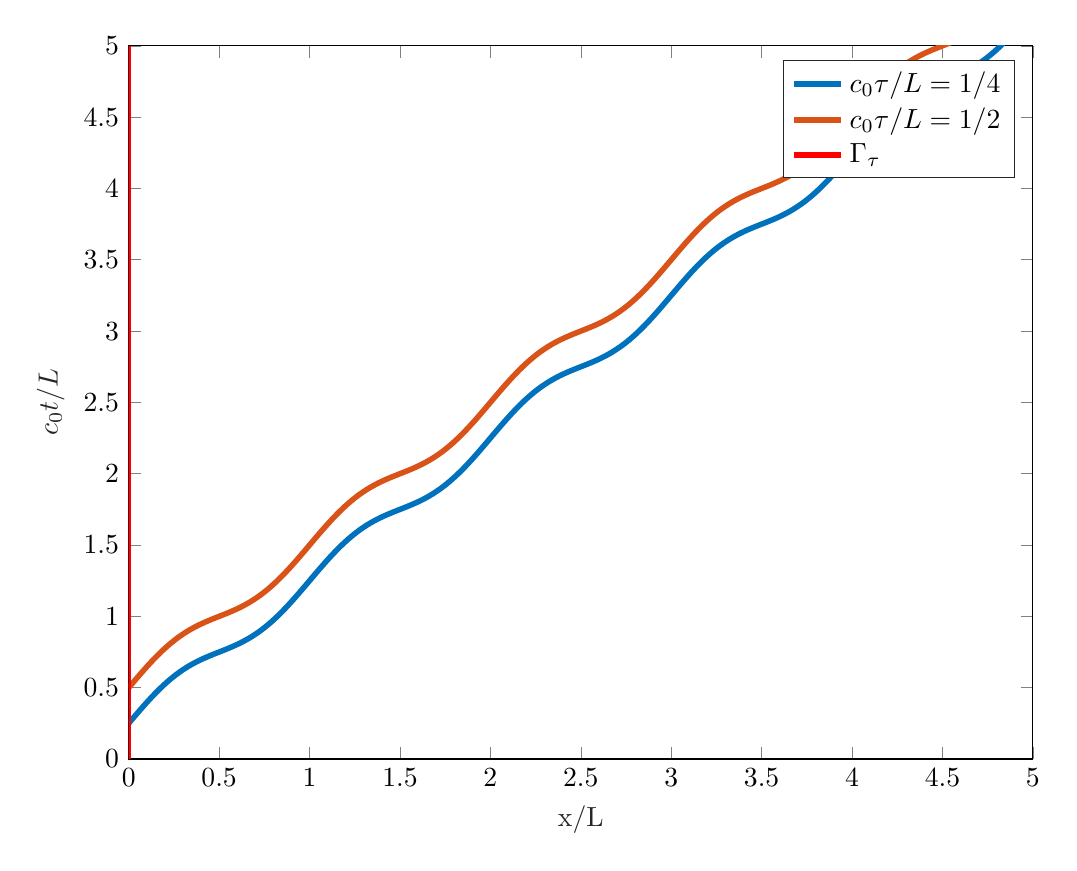
\begin{tikzpicture}

\begin{axis}[%
width=4.521in,
height=3.566in,
at={(0.758in,0.481in)},
scale only axis,
xmin=0,
xmax=5,
xlabel style={font=\color{white!15!black}},
xlabel={x/L},
ymin=0,
ymax=5,
ylabel style={font=\color{white!15!black}},
ylabel={$\text{c}_\text{0}\text{t/L}$},
axis background/.style={fill=white},
legend style={legend cell align=left, align=left, draw=white!15!black}
]
\addplot [color=mycolor1, line width=2.0pt]
  table[row sep=crcr]{%
0	0.25\\
0.01	0.264996710781199\\
0.02	0.279973701827725\\
0.03	0.294911331229688\\
0.04	0.309790112419626\\
0.05	0.324590791077087\\
0.06	0.33929442111663\\
0.07	0.353882439459373\\
0.08	0.368336739292985\\
0.09	0.382639741530997\\
0.1	0.396774464189432\\
0.11	0.410724589406931\\
0.12	0.424474527843901\\
0.13	0.438009480206516\\
0.14	0.451315495652766\\
0.15	0.464379526850061\\
0.16	0.477189481467086\\
0.17	0.489734269896714\\
0.18	0.502003849021618\\
0.19	0.513989261849864\\
0.2	0.525682672864066\\
0.21	0.537077398944598\\
0.22	0.548167935744809\\
0.23	0.558949979414169\\
0.24	0.569420443583596\\
0.25	0.579577471545948\\
0.26	0.589420443583596\\
0.27	0.598949979414169\\
0.28	0.608167935744809\\
0.29	0.617077398944598\\
0.3	0.625682672864066\\
0.31	0.633989261849864\\
0.32	0.642003849021618\\
0.33	0.649734269896714\\
0.34	0.657189481467086\\
0.35	0.664379526850061\\
0.36	0.671315495652766\\
0.37	0.678009480206516\\
0.38	0.684474527843901\\
0.39	0.690724589406931\\
0.4	0.696774464189432\\
0.41	0.702639741530998\\
0.42	0.708336739292985\\
0.43	0.713882439459373\\
0.44	0.71929442111663\\
0.45	0.724590791077087\\
0.46	0.729790112419626\\
0.47	0.734911331229688\\
0.48	0.739973701827725\\
0.49	0.744996710781199\\
0.5	0.75\\
0.51	0.755003289218801\\
0.52	0.760026298172275\\
0.53	0.765088668770312\\
0.54	0.770209887580374\\
0.55	0.775409208922913\\
0.56	0.78070557888337\\
0.57	0.786117560540627\\
0.58	0.791663260707015\\
0.59	0.797360258469002\\
0.6	0.803225535810568\\
0.61	0.809275410593069\\
0.62	0.815525472156099\\
0.63	0.821990519793484\\
0.64	0.828684504347234\\
0.65	0.835620473149939\\
0.66	0.842810518532914\\
0.67	0.850265730103286\\
0.68	0.857996150978382\\
0.69	0.866010738150137\\
0.7	0.874317327135934\\
0.71	0.882922601055402\\
0.72	0.891832064255191\\
0.73	0.901050020585831\\
0.74	0.910579556416404\\
0.75	0.920422528454052\\
0.76	0.930579556416404\\
0.77	0.941050020585831\\
0.78	0.951832064255191\\
0.79	0.962922601055402\\
0.8	0.974317327135934\\
0.81	0.986010738150137\\
0.82	0.997996150978382\\
0.83	1.01026573010329\\
0.84	1.02281051853291\\
0.85	1.03562047314994\\
0.86	1.04868450434723\\
0.87	1.06199051979348\\
0.88	1.0755254721561\\
0.89	1.08927541059307\\
0.9	1.10322553581057\\
0.91	1.117360258469\\
0.92	1.13166326070702\\
0.93	1.14611756054063\\
0.94	1.16070557888337\\
0.95	1.17540920892291\\
0.96	1.19020988758037\\
0.97	1.20508866877031\\
0.98	1.22002629817227\\
0.99	1.2350032892188\\
1	1.25\\
1.01	1.2649967107812\\
1.02	1.27997370182773\\
1.03	1.29491133122969\\
1.04	1.30979011241963\\
1.05	1.32459079107709\\
1.06	1.33929442111663\\
1.07	1.35388243945937\\
1.08	1.36833673929299\\
1.09	1.382639741531\\
1.1	1.39677446418943\\
1.11	1.41072458940693\\
1.12	1.4244745278439\\
1.13	1.43800948020652\\
1.14	1.45131549565277\\
1.15	1.46437952685006\\
1.16	1.47718948146709\\
1.17	1.48973426989671\\
1.18	1.50200384902162\\
1.19	1.51398926184986\\
1.2	1.52568267286407\\
1.21	1.5370773989446\\
1.22	1.54816793574481\\
1.23	1.55894997941417\\
1.24	1.5694204435836\\
1.25	1.57957747154595\\
1.26	1.5894204435836\\
1.27	1.59894997941417\\
1.28	1.60816793574481\\
1.29	1.6170773989446\\
1.3	1.62568267286407\\
1.31	1.63398926184986\\
1.32	1.64200384902162\\
1.33	1.64973426989671\\
1.34	1.65718948146709\\
1.35	1.66437952685006\\
1.36	1.67131549565277\\
1.37	1.67800948020652\\
1.38	1.6844745278439\\
1.39	1.69072458940693\\
1.4	1.69677446418943\\
1.41	1.702639741531\\
1.42	1.70833673929298\\
1.43	1.71388243945937\\
1.44	1.71929442111663\\
1.45	1.72459079107709\\
1.46	1.72979011241963\\
1.47	1.73491133122969\\
1.48	1.73997370182773\\
1.49	1.7449967107812\\
1.5	1.75\\
1.51	1.7550032892188\\
1.52	1.76002629817228\\
1.53	1.76508866877031\\
1.54	1.77020988758037\\
1.55	1.77540920892291\\
1.56	1.78070557888337\\
1.57	1.78611756054063\\
1.58	1.79166326070702\\
1.59	1.797360258469\\
1.6	1.80322553581057\\
1.61	1.80927541059307\\
1.62	1.8155254721561\\
1.63	1.82199051979348\\
1.64	1.82868450434723\\
1.65	1.83562047314994\\
1.66	1.84281051853291\\
1.67	1.85026573010329\\
1.68	1.85799615097838\\
1.69	1.86601073815014\\
1.7	1.87431732713593\\
1.71	1.8829226010554\\
1.72	1.89183206425519\\
1.73	1.90105002058583\\
1.74	1.9105795564164\\
1.75	1.92042252845405\\
1.76	1.9305795564164\\
1.77	1.94105002058583\\
1.78	1.95183206425519\\
1.79	1.9629226010554\\
1.8	1.97431732713593\\
1.81	1.98601073815014\\
1.82	1.99799615097838\\
1.83	2.01026573010329\\
1.84	2.02281051853291\\
1.85	2.03562047314994\\
1.86	2.04868450434723\\
1.87	2.06199051979348\\
1.88	2.0755254721561\\
1.89	2.08927541059307\\
1.9	2.10322553581057\\
1.91	2.117360258469\\
1.92	2.13166326070701\\
1.93	2.14611756054063\\
1.94	2.16070557888337\\
1.95	2.17540920892291\\
1.96	2.19020988758037\\
1.97	2.20508866877031\\
1.98	2.22002629817228\\
1.99	2.2350032892188\\
2	2.25\\
2.01	2.2649967107812\\
2.02	2.27997370182772\\
2.03	2.29491133122969\\
2.04	2.30979011241963\\
2.05	2.32459079107709\\
2.06	2.33929442111663\\
2.07	2.35388243945937\\
2.08	2.36833673929299\\
2.09	2.382639741531\\
2.1	2.39677446418943\\
2.11	2.41072458940693\\
2.12	2.4244745278439\\
2.13	2.43800948020652\\
2.14	2.45131549565277\\
2.15	2.46437952685006\\
2.16	2.47718948146709\\
2.17	2.48973426989671\\
2.18	2.50200384902162\\
2.19	2.51398926184986\\
2.2	2.52568267286407\\
2.21	2.5370773989446\\
2.22	2.54816793574481\\
2.23	2.55894997941417\\
2.24	2.5694204435836\\
2.25	2.57957747154595\\
2.26	2.5894204435836\\
2.27	2.59894997941417\\
2.28	2.60816793574481\\
2.29	2.6170773989446\\
2.3	2.62568267286407\\
2.31	2.63398926184986\\
2.32	2.64200384902162\\
2.33	2.64973426989671\\
2.34	2.65718948146709\\
2.35	2.66437952685006\\
2.36	2.67131549565277\\
2.37	2.67800948020652\\
2.38	2.6844745278439\\
2.39	2.69072458940693\\
2.4	2.69677446418943\\
2.41	2.702639741531\\
2.42	2.70833673929299\\
2.43	2.71388243945937\\
2.44	2.71929442111663\\
2.45	2.72459079107709\\
2.46	2.72979011241963\\
2.47	2.73491133122969\\
2.48	2.73997370182772\\
2.49	2.7449967107812\\
2.5	2.75\\
2.51	2.7550032892188\\
2.52	2.76002629817228\\
2.53	2.76508866877031\\
2.54	2.77020988758037\\
2.55	2.77540920892291\\
2.56	2.78070557888337\\
2.57	2.78611756054063\\
2.58	2.79166326070701\\
2.59	2.797360258469\\
2.6	2.80322553581057\\
2.61	2.80927541059307\\
2.62	2.8155254721561\\
2.63	2.82199051979348\\
2.64	2.82868450434723\\
2.65	2.83562047314994\\
2.66	2.84281051853291\\
2.67	2.85026573010329\\
2.68	2.85799615097838\\
2.69	2.86601073815014\\
2.7	2.87431732713593\\
2.71	2.8829226010554\\
2.72	2.89183206425519\\
2.73	2.90105002058583\\
2.74	2.9105795564164\\
2.75	2.92042252845405\\
2.76	2.9305795564164\\
2.77	2.94105002058583\\
2.78	2.95183206425519\\
2.79	2.9629226010554\\
2.8	2.97431732713593\\
2.81	2.98601073815014\\
2.82	2.99799615097838\\
2.83	3.01026573010329\\
2.84	3.02281051853291\\
2.85	3.03562047314994\\
2.86	3.04868450434723\\
2.87	3.06199051979348\\
2.88	3.0755254721561\\
2.89	3.08927541059307\\
2.9	3.10322553581057\\
2.91	3.117360258469\\
2.92	3.13166326070701\\
2.93	3.14611756054063\\
2.94	3.16070557888337\\
2.95	3.17540920892291\\
2.96	3.19020988758037\\
2.97	3.20508866877031\\
2.98	3.22002629817228\\
2.99	3.2350032892188\\
3	3.25\\
3.01	3.2649967107812\\
3.02	3.27997370182772\\
3.03	3.29491133122969\\
3.04	3.30979011241963\\
3.05	3.32459079107709\\
3.06	3.33929442111663\\
3.07	3.35388243945937\\
3.08	3.36833673929299\\
3.09	3.382639741531\\
3.1	3.39677446418943\\
3.11	3.41072458940693\\
3.12	3.4244745278439\\
3.13	3.43800948020652\\
3.14	3.45131549565277\\
3.15	3.46437952685006\\
3.16	3.47718948146709\\
3.17	3.48973426989671\\
3.18	3.50200384902162\\
3.19	3.51398926184986\\
3.2	3.52568267286407\\
3.21	3.5370773989446\\
3.22	3.54816793574481\\
3.23	3.55894997941417\\
3.24	3.5694204435836\\
3.25	3.57957747154595\\
3.26	3.5894204435836\\
3.27	3.59894997941417\\
3.28	3.60816793574481\\
3.29	3.6170773989446\\
3.3	3.62568267286407\\
3.31	3.63398926184986\\
3.32	3.64200384902162\\
3.33	3.64973426989671\\
3.34	3.65718948146709\\
3.35	3.66437952685006\\
3.36	3.67131549565277\\
3.37	3.67800948020652\\
3.38	3.6844745278439\\
3.39	3.69072458940693\\
3.4	3.69677446418943\\
3.41	3.702639741531\\
3.42	3.70833673929299\\
3.43	3.71388243945937\\
3.44	3.71929442111663\\
3.45	3.72459079107709\\
3.46	3.72979011241963\\
3.47	3.73491133122969\\
3.48	3.73997370182772\\
3.49	3.7449967107812\\
3.5	3.75\\
3.51	3.7550032892188\\
3.52	3.76002629817228\\
3.53	3.76508866877031\\
3.54	3.77020988758037\\
3.55	3.77540920892291\\
3.56	3.78070557888337\\
3.57	3.78611756054063\\
3.58	3.79166326070701\\
3.59	3.797360258469\\
3.6	3.80322553581057\\
3.61	3.80927541059307\\
3.62	3.8155254721561\\
3.63	3.82199051979348\\
3.64	3.82868450434723\\
3.65	3.83562047314994\\
3.66	3.84281051853291\\
3.67	3.85026573010329\\
3.68	3.85799615097838\\
3.69	3.86601073815014\\
3.7	3.87431732713593\\
3.71	3.8829226010554\\
3.72	3.89183206425519\\
3.73	3.90105002058583\\
3.74	3.9105795564164\\
3.75	3.92042252845405\\
3.76	3.9305795564164\\
3.77	3.94105002058583\\
3.78	3.95183206425519\\
3.79	3.9629226010554\\
3.8	3.97431732713593\\
3.81	3.98601073815014\\
3.82	3.99799615097838\\
3.83	4.01026573010329\\
3.84	4.02281051853291\\
3.85	4.03562047314994\\
3.86	4.04868450434723\\
3.87	4.06199051979348\\
3.88	4.0755254721561\\
3.89	4.08927541059307\\
3.9	4.10322553581057\\
3.91	4.117360258469\\
3.92	4.13166326070701\\
3.93	4.14611756054063\\
3.94	4.16070557888337\\
3.95	4.17540920892291\\
3.96	4.19020988758037\\
3.97	4.20508866877031\\
3.98	4.22002629817228\\
3.99	4.2350032892188\\
4	4.25\\
4.01	4.2649967107812\\
4.02	4.27997370182772\\
4.03	4.29491133122969\\
4.04	4.30979011241963\\
4.05	4.32459079107709\\
4.06	4.33929442111663\\
4.07	4.35388243945937\\
4.08	4.36833673929299\\
4.09	4.382639741531\\
4.1	4.39677446418943\\
4.11	4.41072458940693\\
4.12	4.4244745278439\\
4.13	4.43800948020652\\
4.14	4.45131549565277\\
4.15	4.46437952685006\\
4.16	4.47718948146709\\
4.17	4.48973426989671\\
4.18	4.50200384902162\\
4.19	4.51398926184986\\
4.2	4.52568267286407\\
4.21	4.5370773989446\\
4.22	4.54816793574481\\
4.23	4.55894997941417\\
4.24	4.5694204435836\\
4.25	4.57957747154595\\
4.26	4.5894204435836\\
4.27	4.59894997941417\\
4.28	4.60816793574481\\
4.29	4.6170773989446\\
4.3	4.62568267286407\\
4.31	4.63398926184986\\
4.32	4.64200384902162\\
4.33	4.64973426989671\\
4.34	4.65718948146709\\
4.35	4.66437952685006\\
4.36	4.67131549565277\\
4.37	4.67800948020652\\
4.38	4.6844745278439\\
4.39	4.69072458940693\\
4.4	4.69677446418943\\
4.41	4.702639741531\\
4.42	4.70833673929299\\
4.43	4.71388243945937\\
4.44	4.71929442111663\\
4.45	4.72459079107709\\
4.46	4.72979011241963\\
4.47	4.73491133122969\\
4.48	4.73997370182772\\
4.49	4.7449967107812\\
4.5	4.75\\
4.51	4.7550032892188\\
4.52	4.76002629817228\\
4.53	4.76508866877031\\
4.54	4.77020988758037\\
4.55	4.77540920892291\\
4.56	4.78070557888337\\
4.57	4.78611756054063\\
4.58	4.79166326070701\\
4.59	4.797360258469\\
4.6	4.80322553581057\\
4.61	4.80927541059307\\
4.62	4.8155254721561\\
4.63	4.82199051979348\\
4.64	4.82868450434723\\
4.65	4.83562047314994\\
4.66	4.84281051853291\\
4.67	4.85026573010329\\
4.68	4.85799615097838\\
4.69	4.86601073815014\\
4.7	4.87431732713593\\
4.71	4.8829226010554\\
4.72	4.89183206425519\\
4.73	4.90105002058583\\
4.74	4.9105795564164\\
4.75	4.92042252845405\\
4.76	4.9305795564164\\
4.77	4.94105002058583\\
4.78	4.95183206425519\\
4.79	4.9629226010554\\
4.8	4.97431732713593\\
4.81	4.98601073815014\\
4.82	4.99799615097838\\
4.83	5.01026573010329\\
4.84	5.02281051853291\\
4.85	5.03562047314994\\
4.86	5.04868450434723\\
4.87	5.06199051979348\\
4.88	5.0755254721561\\
4.89	5.08927541059307\\
4.9	5.10322553581057\\
4.91	5.117360258469\\
4.92	5.13166326070701\\
4.93	5.14611756054063\\
4.94	5.16070557888337\\
4.95	5.17540920892291\\
4.96	5.19020988758037\\
4.97	5.20508866877031\\
4.98	5.22002629817228\\
4.99	5.2350032892188\\
5	5.25\\
};
\addlegendentry{$\text{c}_\text{0}\tau\text{/L=1/4}$}

\addplot [color=mycolor2, line width=2.0pt]
  table[row sep=crcr]{%
0	0.5\\
0.01	0.514996710781199\\
0.02	0.529973701827725\\
0.03	0.544911331229688\\
0.04	0.559790112419626\\
0.05	0.574590791077087\\
0.06	0.58929442111663\\
0.07	0.603882439459373\\
0.08	0.618336739292985\\
0.09	0.632639741530997\\
0.1	0.646774464189432\\
0.11	0.660724589406931\\
0.12	0.674474527843901\\
0.13	0.688009480206516\\
0.14	0.701315495652766\\
0.15	0.714379526850061\\
0.16	0.727189481467086\\
0.17	0.739734269896714\\
0.18	0.752003849021618\\
0.19	0.763989261849863\\
0.2	0.775682672864066\\
0.21	0.787077398944598\\
0.22	0.798167935744809\\
0.23	0.808949979414169\\
0.24	0.819420443583596\\
0.25	0.829577471545948\\
0.26	0.839420443583596\\
0.27	0.848949979414169\\
0.28	0.858167935744809\\
0.29	0.867077398944598\\
0.3	0.875682672864066\\
0.31	0.883989261849864\\
0.32	0.892003849021618\\
0.33	0.899734269896714\\
0.34	0.907189481467086\\
0.35	0.914379526850061\\
0.36	0.921315495652766\\
0.37	0.928009480206516\\
0.38	0.934474527843901\\
0.39	0.940724589406931\\
0.4	0.946774464189432\\
0.41	0.952639741530998\\
0.42	0.958336739292985\\
0.43	0.963882439459373\\
0.44	0.96929442111663\\
0.45	0.974590791077087\\
0.46	0.979790112419626\\
0.47	0.984911331229688\\
0.48	0.989973701827725\\
0.49	0.994996710781199\\
0.5	1\\
0.51	1.0050032892188\\
0.52	1.01002629817228\\
0.53	1.01508866877031\\
0.54	1.02020988758037\\
0.55	1.02540920892291\\
0.56	1.03070557888337\\
0.57	1.03611756054063\\
0.58	1.04166326070702\\
0.59	1.047360258469\\
0.6	1.05322553581057\\
0.61	1.05927541059307\\
0.62	1.0655254721561\\
0.63	1.07199051979348\\
0.64	1.07868450434723\\
0.65	1.08562047314994\\
0.66	1.09281051853291\\
0.67	1.10026573010329\\
0.68	1.10799615097838\\
0.69	1.11601073815014\\
0.7	1.12431732713593\\
0.71	1.1329226010554\\
0.72	1.14183206425519\\
0.73	1.15105002058583\\
0.74	1.1605795564164\\
0.75	1.17042252845405\\
0.76	1.1805795564164\\
0.77	1.19105002058583\\
0.78	1.20183206425519\\
0.79	1.2129226010554\\
0.8	1.22431732713593\\
0.81	1.23601073815014\\
0.82	1.24799615097838\\
0.83	1.26026573010329\\
0.84	1.27281051853291\\
0.85	1.28562047314994\\
0.86	1.29868450434723\\
0.87	1.31199051979348\\
0.88	1.3255254721561\\
0.89	1.33927541059307\\
0.9	1.35322553581057\\
0.91	1.367360258469\\
0.92	1.38166326070702\\
0.93	1.39611756054063\\
0.94	1.41070557888337\\
0.95	1.42540920892291\\
0.96	1.44020988758037\\
0.97	1.45508866877031\\
0.98	1.47002629817227\\
0.99	1.4850032892188\\
1	1.5\\
1.01	1.5149967107812\\
1.02	1.52997370182773\\
1.03	1.54491133122969\\
1.04	1.55979011241963\\
1.05	1.57459079107709\\
1.06	1.58929442111663\\
1.07	1.60388243945937\\
1.08	1.61833673929299\\
1.09	1.632639741531\\
1.1	1.64677446418943\\
1.11	1.66072458940693\\
1.12	1.6744745278439\\
1.13	1.68800948020652\\
1.14	1.70131549565277\\
1.15	1.71437952685006\\
1.16	1.72718948146709\\
1.17	1.73973426989671\\
1.18	1.75200384902162\\
1.19	1.76398926184986\\
1.2	1.77568267286407\\
1.21	1.7870773989446\\
1.22	1.79816793574481\\
1.23	1.80894997941417\\
1.24	1.8194204435836\\
1.25	1.82957747154595\\
1.26	1.8394204435836\\
1.27	1.84894997941417\\
1.28	1.85816793574481\\
1.29	1.8670773989446\\
1.3	1.87568267286407\\
1.31	1.88398926184986\\
1.32	1.89200384902162\\
1.33	1.89973426989671\\
1.34	1.90718948146709\\
1.35	1.91437952685006\\
1.36	1.92131549565277\\
1.37	1.92800948020652\\
1.38	1.9344745278439\\
1.39	1.94072458940693\\
1.4	1.94677446418943\\
1.41	1.952639741531\\
1.42	1.95833673929298\\
1.43	1.96388243945937\\
1.44	1.96929442111663\\
1.45	1.97459079107709\\
1.46	1.97979011241963\\
1.47	1.98491133122969\\
1.48	1.98997370182773\\
1.49	1.9949967107812\\
1.5	2\\
1.51	2.0050032892188\\
1.52	2.01002629817228\\
1.53	2.01508866877031\\
1.54	2.02020988758037\\
1.55	2.02540920892291\\
1.56	2.03070557888337\\
1.57	2.03611756054063\\
1.58	2.04166326070701\\
1.59	2.047360258469\\
1.6	2.05322553581057\\
1.61	2.05927541059307\\
1.62	2.0655254721561\\
1.63	2.07199051979348\\
1.64	2.07868450434723\\
1.65	2.08562047314994\\
1.66	2.09281051853291\\
1.67	2.10026573010329\\
1.68	2.10799615097838\\
1.69	2.11601073815014\\
1.7	2.12431732713593\\
1.71	2.1329226010554\\
1.72	2.14183206425519\\
1.73	2.15105002058583\\
1.74	2.1605795564164\\
1.75	2.17042252845405\\
1.76	2.1805795564164\\
1.77	2.19105002058583\\
1.78	2.20183206425519\\
1.79	2.2129226010554\\
1.8	2.22431732713593\\
1.81	2.23601073815014\\
1.82	2.24799615097838\\
1.83	2.26026573010329\\
1.84	2.27281051853291\\
1.85	2.28562047314994\\
1.86	2.29868450434723\\
1.87	2.31199051979348\\
1.88	2.3255254721561\\
1.89	2.33927541059307\\
1.9	2.35322553581057\\
1.91	2.367360258469\\
1.92	2.38166326070701\\
1.93	2.39611756054063\\
1.94	2.41070557888337\\
1.95	2.42540920892291\\
1.96	2.44020988758037\\
1.97	2.45508866877031\\
1.98	2.47002629817228\\
1.99	2.4850032892188\\
2	2.5\\
2.01	2.5149967107812\\
2.02	2.52997370182772\\
2.03	2.54491133122969\\
2.04	2.55979011241963\\
2.05	2.57459079107709\\
2.06	2.58929442111663\\
2.07	2.60388243945937\\
2.08	2.61833673929299\\
2.09	2.632639741531\\
2.1	2.64677446418943\\
2.11	2.66072458940693\\
2.12	2.6744745278439\\
2.13	2.68800948020652\\
2.14	2.70131549565277\\
2.15	2.71437952685006\\
2.16	2.72718948146709\\
2.17	2.73973426989671\\
2.18	2.75200384902162\\
2.19	2.76398926184986\\
2.2	2.77568267286407\\
2.21	2.7870773989446\\
2.22	2.79816793574481\\
2.23	2.80894997941417\\
2.24	2.8194204435836\\
2.25	2.82957747154595\\
2.26	2.8394204435836\\
2.27	2.84894997941417\\
2.28	2.85816793574481\\
2.29	2.8670773989446\\
2.3	2.87568267286407\\
2.31	2.88398926184986\\
2.32	2.89200384902162\\
2.33	2.89973426989671\\
2.34	2.90718948146709\\
2.35	2.91437952685006\\
2.36	2.92131549565277\\
2.37	2.92800948020652\\
2.38	2.9344745278439\\
2.39	2.94072458940693\\
2.4	2.94677446418943\\
2.41	2.952639741531\\
2.42	2.95833673929299\\
2.43	2.96388243945937\\
2.44	2.96929442111663\\
2.45	2.97459079107709\\
2.46	2.97979011241963\\
2.47	2.98491133122969\\
2.48	2.98997370182772\\
2.49	2.9949967107812\\
2.5	3\\
2.51	3.0050032892188\\
2.52	3.01002629817228\\
2.53	3.01508866877031\\
2.54	3.02020988758037\\
2.55	3.02540920892291\\
2.56	3.03070557888337\\
2.57	3.03611756054063\\
2.58	3.04166326070701\\
2.59	3.047360258469\\
2.6	3.05322553581057\\
2.61	3.05927541059307\\
2.62	3.0655254721561\\
2.63	3.07199051979348\\
2.64	3.07868450434723\\
2.65	3.08562047314994\\
2.66	3.09281051853291\\
2.67	3.10026573010329\\
2.68	3.10799615097838\\
2.69	3.11601073815014\\
2.7	3.12431732713593\\
2.71	3.1329226010554\\
2.72	3.14183206425519\\
2.73	3.15105002058583\\
2.74	3.1605795564164\\
2.75	3.17042252845405\\
2.76	3.1805795564164\\
2.77	3.19105002058583\\
2.78	3.20183206425519\\
2.79	3.2129226010554\\
2.8	3.22431732713593\\
2.81	3.23601073815014\\
2.82	3.24799615097838\\
2.83	3.26026573010329\\
2.84	3.27281051853291\\
2.85	3.28562047314994\\
2.86	3.29868450434723\\
2.87	3.31199051979348\\
2.88	3.3255254721561\\
2.89	3.33927541059307\\
2.9	3.35322553581057\\
2.91	3.367360258469\\
2.92	3.38166326070701\\
2.93	3.39611756054063\\
2.94	3.41070557888337\\
2.95	3.42540920892291\\
2.96	3.44020988758037\\
2.97	3.45508866877031\\
2.98	3.47002629817228\\
2.99	3.4850032892188\\
3	3.5\\
3.01	3.5149967107812\\
3.02	3.52997370182772\\
3.03	3.54491133122969\\
3.04	3.55979011241963\\
3.05	3.57459079107709\\
3.06	3.58929442111663\\
3.07	3.60388243945937\\
3.08	3.61833673929299\\
3.09	3.632639741531\\
3.1	3.64677446418943\\
3.11	3.66072458940693\\
3.12	3.6744745278439\\
3.13	3.68800948020652\\
3.14	3.70131549565277\\
3.15	3.71437952685006\\
3.16	3.72718948146709\\
3.17	3.73973426989671\\
3.18	3.75200384902162\\
3.19	3.76398926184986\\
3.2	3.77568267286407\\
3.21	3.7870773989446\\
3.22	3.79816793574481\\
3.23	3.80894997941417\\
3.24	3.8194204435836\\
3.25	3.82957747154595\\
3.26	3.8394204435836\\
3.27	3.84894997941417\\
3.28	3.85816793574481\\
3.29	3.8670773989446\\
3.3	3.87568267286407\\
3.31	3.88398926184986\\
3.32	3.89200384902162\\
3.33	3.89973426989671\\
3.34	3.90718948146709\\
3.35	3.91437952685006\\
3.36	3.92131549565277\\
3.37	3.92800948020652\\
3.38	3.9344745278439\\
3.39	3.94072458940693\\
3.4	3.94677446418943\\
3.41	3.952639741531\\
3.42	3.95833673929299\\
3.43	3.96388243945937\\
3.44	3.96929442111663\\
3.45	3.97459079107709\\
3.46	3.97979011241963\\
3.47	3.98491133122969\\
3.48	3.98997370182772\\
3.49	3.9949967107812\\
3.5	4\\
3.51	4.0050032892188\\
3.52	4.01002629817227\\
3.53	4.01508866877031\\
3.54	4.02020988758037\\
3.55	4.02540920892291\\
3.56	4.03070557888337\\
3.57	4.03611756054063\\
3.58	4.04166326070701\\
3.59	4.047360258469\\
3.6	4.05322553581057\\
3.61	4.05927541059307\\
3.62	4.0655254721561\\
3.63	4.07199051979348\\
3.64	4.07868450434723\\
3.65	4.08562047314994\\
3.66	4.09281051853291\\
3.67	4.10026573010329\\
3.68	4.10799615097838\\
3.69	4.11601073815014\\
3.7	4.12431732713593\\
3.71	4.1329226010554\\
3.72	4.14183206425519\\
3.73	4.15105002058583\\
3.74	4.1605795564164\\
3.75	4.17042252845405\\
3.76	4.1805795564164\\
3.77	4.19105002058583\\
3.78	4.20183206425519\\
3.79	4.2129226010554\\
3.8	4.22431732713593\\
3.81	4.23601073815014\\
3.82	4.24799615097838\\
3.83	4.26026573010329\\
3.84	4.27281051853291\\
3.85	4.28562047314994\\
3.86	4.29868450434723\\
3.87	4.31199051979348\\
3.88	4.3255254721561\\
3.89	4.33927541059307\\
3.9	4.35322553581057\\
3.91	4.367360258469\\
3.92	4.38166326070701\\
3.93	4.39611756054063\\
3.94	4.41070557888337\\
3.95	4.42540920892291\\
3.96	4.44020988758037\\
3.97	4.45508866877031\\
3.98	4.47002629817228\\
3.99	4.4850032892188\\
4	4.5\\
4.01	4.5149967107812\\
4.02	4.52997370182772\\
4.03	4.54491133122969\\
4.04	4.55979011241963\\
4.05	4.57459079107709\\
4.06	4.58929442111663\\
4.07	4.60388243945937\\
4.08	4.61833673929299\\
4.09	4.632639741531\\
4.1	4.64677446418943\\
4.11	4.66072458940693\\
4.12	4.6744745278439\\
4.13	4.68800948020652\\
4.14	4.70131549565277\\
4.15	4.71437952685006\\
4.16	4.72718948146709\\
4.17	4.73973426989671\\
4.18	4.75200384902162\\
4.19	4.76398926184986\\
4.2	4.77568267286407\\
4.21	4.7870773989446\\
4.22	4.79816793574481\\
4.23	4.80894997941417\\
4.24	4.8194204435836\\
4.25	4.82957747154595\\
4.26	4.8394204435836\\
4.27	4.84894997941417\\
4.28	4.85816793574481\\
4.29	4.8670773989446\\
4.3	4.87568267286407\\
4.31	4.88398926184986\\
4.32	4.89200384902162\\
4.33	4.89973426989671\\
4.34	4.90718948146709\\
4.35	4.91437952685006\\
4.36	4.92131549565277\\
4.37	4.92800948020652\\
4.38	4.9344745278439\\
4.39	4.94072458940693\\
4.4	4.94677446418943\\
4.41	4.952639741531\\
4.42	4.95833673929299\\
4.43	4.96388243945937\\
4.44	4.96929442111663\\
4.45	4.97459079107709\\
4.46	4.97979011241963\\
4.47	4.98491133122969\\
4.48	4.98997370182772\\
4.49	4.9949967107812\\
4.5	5\\
4.51	5.0050032892188\\
4.52	5.01002629817228\\
4.53	5.01508866877031\\
4.54	5.02020988758037\\
4.55	5.02540920892291\\
4.56	5.03070557888337\\
4.57	5.03611756054063\\
4.58	5.04166326070701\\
4.59	5.047360258469\\
4.6	5.05322553581057\\
4.61	5.05927541059307\\
4.62	5.0655254721561\\
4.63	5.07199051979348\\
4.64	5.07868450434723\\
4.65	5.08562047314994\\
4.66	5.09281051853291\\
4.67	5.10026573010329\\
4.68	5.10799615097838\\
4.69	5.11601073815014\\
4.7	5.12431732713593\\
4.71	5.1329226010554\\
4.72	5.14183206425519\\
4.73	5.15105002058583\\
4.74	5.1605795564164\\
4.75	5.17042252845405\\
4.76	5.1805795564164\\
4.77	5.19105002058583\\
4.78	5.20183206425519\\
4.79	5.2129226010554\\
4.8	5.22431732713593\\
4.81	5.23601073815014\\
4.82	5.24799615097838\\
4.83	5.26026573010329\\
4.84	5.27281051853291\\
4.85	5.28562047314994\\
4.86	5.29868450434723\\
4.87	5.31199051979348\\
4.88	5.3255254721561\\
4.89	5.33927541059307\\
4.9	5.35322553581057\\
4.91	5.367360258469\\
4.92	5.38166326070701\\
4.93	5.39611756054063\\
4.94	5.41070557888337\\
4.95	5.42540920892291\\
4.96	5.44020988758037\\
4.97	5.45508866877031\\
4.98	5.47002629817228\\
4.99	5.4850032892188\\
5	5.5\\
};
\addlegendentry{$\text{c}_\text{0}\tau\text{/L=1/2}$}

\addplot [color=red, line width=2.0pt]
  table[row sep=crcr]{%
0	0\\
0	0.01\\
0	0.02\\
0	0.03\\
0	0.04\\
0	0.05\\
0	0.06\\
0	0.07\\
0	0.08\\
0	0.09\\
0	0.1\\
0	0.11\\
0	0.12\\
0	0.13\\
0	0.14\\
0	0.15\\
0	0.16\\
0	0.17\\
0	0.18\\
0	0.19\\
0	0.2\\
0	0.21\\
0	0.22\\
0	0.23\\
0	0.24\\
0	0.25\\
0	0.26\\
0	0.27\\
0	0.28\\
0	0.29\\
0	0.3\\
0	0.31\\
0	0.32\\
0	0.33\\
0	0.34\\
0	0.35\\
0	0.36\\
0	0.37\\
0	0.38\\
0	0.39\\
0	0.4\\
0	0.41\\
0	0.42\\
0	0.43\\
0	0.44\\
0	0.45\\
0	0.46\\
0	0.47\\
0	0.48\\
0	0.49\\
0	0.5\\
0	0.51\\
0	0.52\\
0	0.53\\
0	0.54\\
0	0.55\\
0	0.56\\
0	0.57\\
0	0.58\\
0	0.59\\
0	0.6\\
0	0.61\\
0	0.62\\
0	0.63\\
0	0.64\\
0	0.65\\
0	0.66\\
0	0.67\\
0	0.68\\
0	0.69\\
0	0.7\\
0	0.71\\
0	0.72\\
0	0.73\\
0	0.74\\
0	0.75\\
0	0.76\\
0	0.77\\
0	0.78\\
0	0.79\\
0	0.8\\
0	0.81\\
0	0.82\\
0	0.83\\
0	0.84\\
0	0.85\\
0	0.86\\
0	0.87\\
0	0.88\\
0	0.89\\
0	0.9\\
0	0.91\\
0	0.92\\
0	0.93\\
0	0.94\\
0	0.95\\
0	0.96\\
0	0.97\\
0	0.98\\
0	0.99\\
0	1\\
0	1.01\\
0	1.02\\
0	1.03\\
0	1.04\\
0	1.05\\
0	1.06\\
0	1.07\\
0	1.08\\
0	1.09\\
0	1.1\\
0	1.11\\
0	1.12\\
0	1.13\\
0	1.14\\
0	1.15\\
0	1.16\\
0	1.17\\
0	1.18\\
0	1.19\\
0	1.2\\
0	1.21\\
0	1.22\\
0	1.23\\
0	1.24\\
0	1.25\\
0	1.26\\
0	1.27\\
0	1.28\\
0	1.29\\
0	1.3\\
0	1.31\\
0	1.32\\
0	1.33\\
0	1.34\\
0	1.35\\
0	1.36\\
0	1.37\\
0	1.38\\
0	1.39\\
0	1.4\\
0	1.41\\
0	1.42\\
0	1.43\\
0	1.44\\
0	1.45\\
0	1.46\\
0	1.47\\
0	1.48\\
0	1.49\\
0	1.5\\
0	1.51\\
0	1.52\\
0	1.53\\
0	1.54\\
0	1.55\\
0	1.56\\
0	1.57\\
0	1.58\\
0	1.59\\
0	1.6\\
0	1.61\\
0	1.62\\
0	1.63\\
0	1.64\\
0	1.65\\
0	1.66\\
0	1.67\\
0	1.68\\
0	1.69\\
0	1.7\\
0	1.71\\
0	1.72\\
0	1.73\\
0	1.74\\
0	1.75\\
0	1.76\\
0	1.77\\
0	1.78\\
0	1.79\\
0	1.8\\
0	1.81\\
0	1.82\\
0	1.83\\
0	1.84\\
0	1.85\\
0	1.86\\
0	1.87\\
0	1.88\\
0	1.89\\
0	1.9\\
0	1.91\\
0	1.92\\
0	1.93\\
0	1.94\\
0	1.95\\
0	1.96\\
0	1.97\\
0	1.98\\
0	1.99\\
0	2\\
0	2.01\\
0	2.02\\
0	2.03\\
0	2.04\\
0	2.05\\
0	2.06\\
0	2.07\\
0	2.08\\
0	2.09\\
0	2.1\\
0	2.11\\
0	2.12\\
0	2.13\\
0	2.14\\
0	2.15\\
0	2.16\\
0	2.17\\
0	2.18\\
0	2.19\\
0	2.2\\
0	2.21\\
0	2.22\\
0	2.23\\
0	2.24\\
0	2.25\\
0	2.26\\
0	2.27\\
0	2.28\\
0	2.29\\
0	2.3\\
0	2.31\\
0	2.32\\
0	2.33\\
0	2.34\\
0	2.35\\
0	2.36\\
0	2.37\\
0	2.38\\
0	2.39\\
0	2.4\\
0	2.41\\
0	2.42\\
0	2.43\\
0	2.44\\
0	2.45\\
0	2.46\\
0	2.47\\
0	2.48\\
0	2.49\\
0	2.5\\
0	2.51\\
0	2.52\\
0	2.53\\
0	2.54\\
0	2.55\\
0	2.56\\
0	2.57\\
0	2.58\\
0	2.59\\
0	2.6\\
0	2.61\\
0	2.62\\
0	2.63\\
0	2.64\\
0	2.65\\
0	2.66\\
0	2.67\\
0	2.68\\
0	2.69\\
0	2.7\\
0	2.71\\
0	2.72\\
0	2.73\\
0	2.74\\
0	2.75\\
0	2.76\\
0	2.77\\
0	2.78\\
0	2.79\\
0	2.8\\
0	2.81\\
0	2.82\\
0	2.83\\
0	2.84\\
0	2.85\\
0	2.86\\
0	2.87\\
0	2.88\\
0	2.89\\
0	2.9\\
0	2.91\\
0	2.92\\
0	2.93\\
0	2.94\\
0	2.95\\
0	2.96\\
0	2.97\\
0	2.98\\
0	2.99\\
0	3\\
0	3.01\\
0	3.02\\
0	3.03\\
0	3.04\\
0	3.05\\
0	3.06\\
0	3.07\\
0	3.08\\
0	3.09\\
0	3.1\\
0	3.11\\
0	3.12\\
0	3.13\\
0	3.14\\
0	3.15\\
0	3.16\\
0	3.17\\
0	3.18\\
0	3.19\\
0	3.2\\
0	3.21\\
0	3.22\\
0	3.23\\
0	3.24\\
0	3.25\\
0	3.26\\
0	3.27\\
0	3.28\\
0	3.29\\
0	3.3\\
0	3.31\\
0	3.32\\
0	3.33\\
0	3.34\\
0	3.35\\
0	3.36\\
0	3.37\\
0	3.38\\
0	3.39\\
0	3.4\\
0	3.41\\
0	3.42\\
0	3.43\\
0	3.44\\
0	3.45\\
0	3.46\\
0	3.47\\
0	3.48\\
0	3.49\\
0	3.5\\
0	3.51\\
0	3.52\\
0	3.53\\
0	3.54\\
0	3.55\\
0	3.56\\
0	3.57\\
0	3.58\\
0	3.59\\
0	3.6\\
0	3.61\\
0	3.62\\
0	3.63\\
0	3.64\\
0	3.65\\
0	3.66\\
0	3.67\\
0	3.68\\
0	3.69\\
0	3.7\\
0	3.71\\
0	3.72\\
0	3.73\\
0	3.74\\
0	3.75\\
0	3.76\\
0	3.77\\
0	3.78\\
0	3.79\\
0	3.8\\
0	3.81\\
0	3.82\\
0	3.83\\
0	3.84\\
0	3.85\\
0	3.86\\
0	3.87\\
0	3.88\\
0	3.89\\
0	3.9\\
0	3.91\\
0	3.92\\
0	3.93\\
0	3.94\\
0	3.95\\
0	3.96\\
0	3.97\\
0	3.98\\
0	3.99\\
0	4\\
0	4.01\\
0	4.02\\
0	4.03\\
0	4.04\\
0	4.05\\
0	4.06\\
0	4.07\\
0	4.08\\
0	4.09\\
0	4.1\\
0	4.11\\
0	4.12\\
0	4.13\\
0	4.14\\
0	4.15\\
0	4.16\\
0	4.17\\
0	4.18\\
0	4.19\\
0	4.2\\
0	4.21\\
0	4.22\\
0	4.23\\
0	4.24\\
0	4.25\\
0	4.26\\
0	4.27\\
0	4.28\\
0	4.29\\
0	4.3\\
0	4.31\\
0	4.32\\
0	4.33\\
0	4.34\\
0	4.35\\
0	4.36\\
0	4.37\\
0	4.38\\
0	4.39\\
0	4.4\\
0	4.41\\
0	4.42\\
0	4.43\\
0	4.44\\
0	4.45\\
0	4.46\\
0	4.47\\
0	4.48\\
0	4.49\\
0	4.5\\
0	4.51\\
0	4.52\\
0	4.53\\
0	4.54\\
0	4.55\\
0	4.56\\
0	4.57\\
0	4.58\\
0	4.59\\
0	4.6\\
0	4.61\\
0	4.62\\
0	4.63\\
0	4.64\\
0	4.65\\
0	4.66\\
0	4.67\\
0	4.68\\
0	4.69\\
0	4.7\\
0	4.71\\
0	4.72\\
0	4.73\\
0	4.74\\
0	4.75\\
0	4.76\\
0	4.77\\
0	4.78\\
0	4.79\\
0	4.8\\
0	4.81\\
0	4.82\\
0	4.83\\
0	4.84\\
0	4.85\\
0	4.86\\
0	4.87\\
0	4.88\\
0	4.89\\
0	4.9\\
0	4.91\\
0	4.92\\
0	4.93\\
0	4.94\\
0	4.95\\
0	4.96\\
0	4.97\\
0	4.98\\
0	4.99\\
0	5\\
};
\addlegendentry{$\Gamma{}_\tau$}

\end{axis}
\end{tikzpicture}%
		%\caption{}
	\end{solfig}
	
	\item L'équation des caractéristiques établie avant est 
	$$\frac{x}{L}+\frac{1}{4\pi}\sin(2\pi x/L) -\frac{s}{L}-\frac{1}{4\pi}\sin(2\pi s/L) =\frac{c_0 t}{L} ,$$
	on ne peut pas isoler $s$ dans cette équation en $s$ et $\sin(s)$, c'est donc une équation implicite à résoudre numériquement.
	
	\item L'équation devient 
	$$ 
	c(x)\frac{\partial u}{\partial x}+\frac{\partial u}{\partial t}=\frac{cu}{L}-c'(x)u,
	$$ 
	on peut alors la résoudre en intégrant la relation $R \mbox{d} x= P \mbox{d} u$ le long des caractéristiques émanant de la courbe $\Gamma$ et situées dans la région A.
	$$
		\int_s^x (\frac{c(\overline{x})\overline{u}}{L}-c'(\overline{x})\overline{u}) \:\mbox{d} \overline{x}=\int_{u(s,0)}^{u(x,t)} c(\overline{x}) \: \mbox{d} \overline{u}
	$$
	$$
	\int_s^x (\frac{1}{L}-\frac{c'(\overline{x})}{c(\overline{x})}) \:\mbox{d} \overline{x}=\int_{u(s,0)}^{u(x,t)}  \frac{\mbox{d} \overline{u}}{\overline{u}}
	$$
	$$     \frac{x-s}{L}-\ln(\frac{c(x)}{c(s)})=\ln(\frac{u(x,t)}{u(s,0)})$$
	$$   \Rightarrow u(x,t)=u_0 e^\frac{x-s}{L} \frac{1+\frac{1}{2}\cos(2\pi x/L)}{1+\frac{1}{2}\cos(2\pi s/L)}\frac{s/L_0}{1+(s/L_0)^3}$$
	Cette solution contient encore la variable $s(x,t)$ qui doit être remplacée par la solution de l'équation implicite établie au point 2. 
	
\end{enumerate}	
	
\end{solution}


\section{}

On considère l'EDP suivante pour $u(x,t)$:
$$ 
\frac{\partial u}{\partial t}=\alpha \frac{\partial^2 u}{\partial x^2}+Q_0\cos(\frac{\pi}{2}\frac{x}{L})
$$
avec $\alpha>0$ et $Q_0$ constants.\\
Le domaine est borné: $0\leqslant x\leqslant L$.
La condition initiale est $$u(x,0)=u_0(2x/L-1)$$ avec $u_0>0$ constant.\\ Les conditions aux limites sont $\frac{\partial u}{\partial x}(0,t)=2u_0/L$ et $u(L,t)=u_0$.

\begin{enumerate}
	\item De quel type d'EDP s'agit-il, physiquement ET mathématiquement? Qu'est-ce qu'un temps \textit{court} pour une telle EDP : $0\leqslant t<<...$ ?
	\item La solution est de la forme $u(x,t) = R(x) + \Theta(x,t)$ avec $R$ la solution de régime et $\Theta$ la solution transitoire. 
	\begin{itemize}
		\item Obtenez d'abord $R$
		\item Obtenez ensuite $\Theta$ en utilisant la méthode de séparation des variables
	\end{itemize}
	
	\item On considère le cas particulier $$Q_0=(\pi/2)^2\frac{\alpha\: u_0}{L^2}.$$ Esquissez (proprement avec des axes chiffrés) le graphe attendu de $u/u_0$ en fonction de $x/L$ pour des temps différents: $t=0$ (CI), temps \textit{court}, temps \textit{moyen}, temps \textit{très long} (solution de régime).
\end{enumerate}


\begin{solution}
	
	\begin{enumerate}
		\item Il s'agit d'une équation parabolique (mathématiquement) et plus particulièrement de l'équation de diffusion (physiquement) avec un terme source, elle modélise par exemple un transfert de chaleur. Un temps court pour cette EDP, comme on le verra par la suite, est un temps pour lequel la solution n'a pas encore atteint sa valeur de régime, c'est-à-dire $t<L^2/\alpha$. En effet, $\alpha$ s'exprime en $m^2/s$, c'est donc la seule combinaison qui permet d'obtenir les mêmes unités que $t$. C'est peu probable qu'un facteur multiplicatif soit présent mais il est possible que $4L^2/(\pi^2\alpha)$ soit plus approprié en analysant la solution finale et le graphe de la solution.
		
		\item On remplace $u$ par $R(x)$ dans l'équation
		$$\alpha R''(x)+Q_0\cos\Big(\frac{\pi}{2}\frac{x}{L}\Big)=0 \Longrightarrow R(x)=Ax+B+\frac{Q_0}{\alpha}\Big(\frac{2L}{\pi}\Big)^2\cos\Big(\frac{\pi}{2}\frac{x}{L}\Big)\qquad A,B\in \Re$$
		On détermine A et B par les conditions limites:
		$$R'(0)=\frac{2u_0}{L}\Longrightarrow A=\frac{2u_0}{L}$$
		$$R(L)=AL+B=u_0\Longrightarrow B=-u_0$$
		$$\Longrightarrow R(x)=u_0(2x/L-1)+\frac{Q_0}{\alpha}\Big(\frac{2L}{\pi}\Big)^2\cos\Big(\frac{\pi}{2}\frac{x}{L}\Big)$$
		On calcule ensuite $\Theta(x,t)=X(x)T(t)$ en remplaçant $u$ par $\Theta$:
		$$\frac{T'}{\alpha T}=\frac{X''}{X}$$
		Puisque la partie gauche ne dépend que de $t$ et celle de droite ne dépend que de $x$, elle sont constantes et valent $0,k^2$ ou $-k^2$. Seul le cas $-k^2$ conduit à une solution non nulle:
		$$\frac{T'(t)}{T(t)}=-\alpha k^2\Longrightarrow T(t)=Ce^{-\alpha k^2 t}\qquad C\in \Re$$
		$$\frac{X''(x)}{X(x)}=-k^2 \Longrightarrow X(x)=D\cos(kx) +E\sin(kx) \qquad D,E\in \Re$$
		Puisque les conditions limites sont respectées par la solution de régime, ces conditions doivent être nulles pour la solution transitoire (sinon, les conditions aux frontières pour $u$ vaudraient 2 fois celles imposées par le problème). On résout donc les conditions homogènes pour trouver C,D et E.
		$$  \frac{\partial \Theta}{\partial x}(0,t)=X'(0)T(t)=0\Longrightarrow E=0 $$
		$$\Theta(L,t)=X(L)T(t)=0\Longrightarrow CD\cos(kL)=0\Longrightarrow kL=\Big(n+\frac{1}{2}\Big)\pi$$
		$$k_n=\Big(n+\frac{1}{2}\Big)\frac{\pi}{L}\qquad n=0,1,2,...$$
		On a donc comme solution transitoire
		$$\Theta(x,t)=\sum_{n=0}^{\infty} F_n e^{-\alpha k_n^2 t}\cos\Big(\Big(n+\frac{1}{2}\Big)\frac{\pi x}{L}\Big)$$
		avec $F_n=(CD)_n$.
		Il reste à trouver les constantes $F_n$ grâce à la condition initiale.
		$$\Theta(x,t=0)=u(x,0)-R(x)$$
		$$ \sum_{n=0}^{\infty} F_n \cos\Big(\Big(n+\frac{1}{2}\Big)\frac{\pi x}{L}\Big)=-\frac{Q_0}{\alpha}\Big(\frac{2L}{\pi}\Big)^2\cos\Big(\frac{\pi}{2}\frac{x}{L}\Big)  $$
		Par chance, la condition initiale est une fonction cosinus, les termes $F_n$ de la série de Fourier ne forment pas une suite infinie. Il suffit de prendre $$F_0=-\frac{Q_0}{\alpha}\Big(\frac{2L}{\pi}\Big)^2$$
		pour $n=0$ et $F_n=0$ pour $n>0$. Il n'est donc pas nécessaire d'utiliser la propriété d'orthogonalité des cosinus. Si vous avez quand même essayé d'intégrer en multipliant par le cosinus, vous auriez obtenu une somme de $\frac{1}{n}\sin(...x)$ et $\frac{1}{n+1}\sin(...x)$. Cette somme s'annule toujours sauf quand le dénominateur est nul ($n=0$) et on retombe sur le bon résultat.\\
		Finalement,
		$$ \Theta(x,t)= -\frac{Q_0}{\alpha}\Big(\frac{2L}{\pi}\Big)^2e^{-\frac{\pi^2\alpha}{4L^2} t}\cos\Big(\frac{\pi x}{2L}\Big)$$
		
		\item Avec le cas particulier, la solution finale vaut 
		$$\frac{u(x,t)}{u_0}=\frac{2x}{L}-1+\cos\Big(\frac{\pi x}{2L}\Big)\Big( 1-e^{-\frac{\pi^2\alpha}{4L^2} t} \Big)$$
		Les 2 graphes suivants présentent la solution.
		
		\begin{solfig}{c}{Solution $u/u_0$}
			\centering
			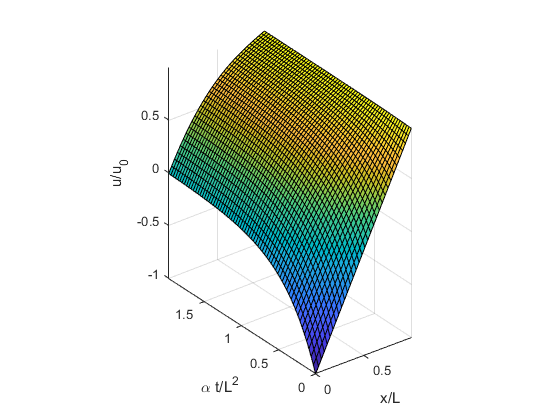
\includegraphics[scale = 0.6]{aout2017-4.png}
			%\caption{}
		\end{solfig}
		
		\begin{solfig}{c}{Solution $u/u_0$ pour des temps différents}
			\centering
			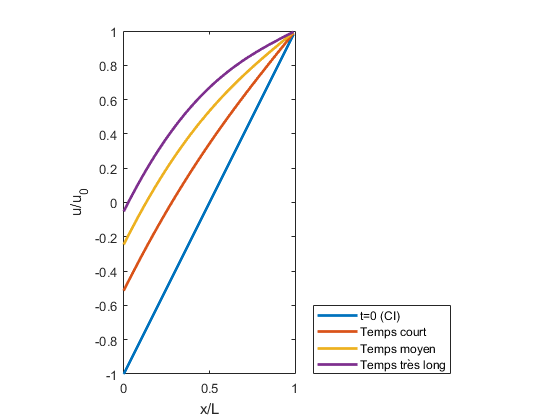
\includegraphics[scale = 0.8]{aout2017-5.png}
			%\caption{}
		\end{solfig}
	\end{enumerate}
	
	
	
\end{solution}


\section{}

On considère la fonction
$$f(z)=\frac{e^{-i/z}}{z}$$
\begin{enumerate}
	\item Calculez le résidu de $f(z)$ en $z=0$.
	\item Donnez les points singuliers de $f(z)$ et précisez leur type.
\end{enumerate}

\begin{solution}
	
	\begin{enumerate}
		\item On calcule le développement en série de Laurent de $f(z)$:
		$$ e^y=1+y+\frac{y^2}{2}+\frac{y^3}{6}+... $$
		$$ e^{-i/z}=1-\frac{i}{z}-\frac{1}{2z^2}+\frac{i}{6z^3}+... $$
		$$ \frac{e^{-i/z}}{z}=\frac{1}{z}-\frac{i}{z^2}-\frac{1}{2z^3}+\frac{i}{6z^4}+... $$
		Le résidu en $z=0$ est le coefficient du terme en $1/z$ de la série de Laurent et vaut donc 1. 
		\item $z=0$ est le seul point où $f(z)$ n'est pas dérivable. Puisqu'on peut trouver un voisinage dans lequel le point $z=0$ est le seul point singulier, ce point est un point singulier isolé. De plus, c'est un point singulier essentiel car $1/f(z)$ n'est pas bornée au voisinage de ce point:\\
		\begin{itemize}
			\item $f(z)$ n'est pas dérivable en 0 car elle n'est pas continue en ce point. Elle n'est pas bornée (et donc pas continue) en arrivant par le chemin $\Re(z)=0$ et $\Im (z)<0$: $$\lim_{y\rightarrow 0^-,x=0} f(z)=\lim_{y\rightarrow 0^-,x=0} \frac{e^{-i/(x+iy)}}{x+iy}=\lim_{y\rightarrow 0^-,x=0} \frac{e^{-1/y}}{iy}=\frac{e^{-1/0^-}}{i0^-}=-i\frac{\infty}{0^-}=+\infty\:i.$$
			\item $1/f(z)$ n'est pas bornée autour de 0 suivant le chemin $\Re(z)=0$ et $\Im (z)>0$: $$\lim_{y\rightarrow 0^+,x=0} 1/f(z)=\lim_{y\rightarrow 0^+,x=0} (x+iy)e^{i/(x+iy)}=\lim_{y\rightarrow 0^+,x=0}iye^{1/y}$$ $$=\lim_{y\rightarrow 0^+,x=0}\frac{ie^{1/y}}{1/y}\overset{\infty/\infty}{=}\lim_{y\rightarrow 0^+,x=0}\frac{-ie^{1/y}/y^2}{-1/y^2}=\lim_{y\rightarrow 0^+,x=0}ie^{1/0^+}=+\infty\:i.$$
			Il faut faire attention à vérifier la valeur de la fonction pour tout chemin passant par l'origine. En effet, la fonction tend vers 0 pour les 3 autres chemins principaux: venant de l'axe réel négatif, venant de l'axe réel positif et venant de l'axe imaginaire négatif.
		\end{itemize}
		
		Le fait que la série de Laurent ne soit pas limitée du côté des puissances négatives confirme qu'il ne s'agit pas d'un pôle.
		
		\begin{solfig}{c}{Graphe de $1/f(z)$ aux environs de $z=0$}
			\centering
			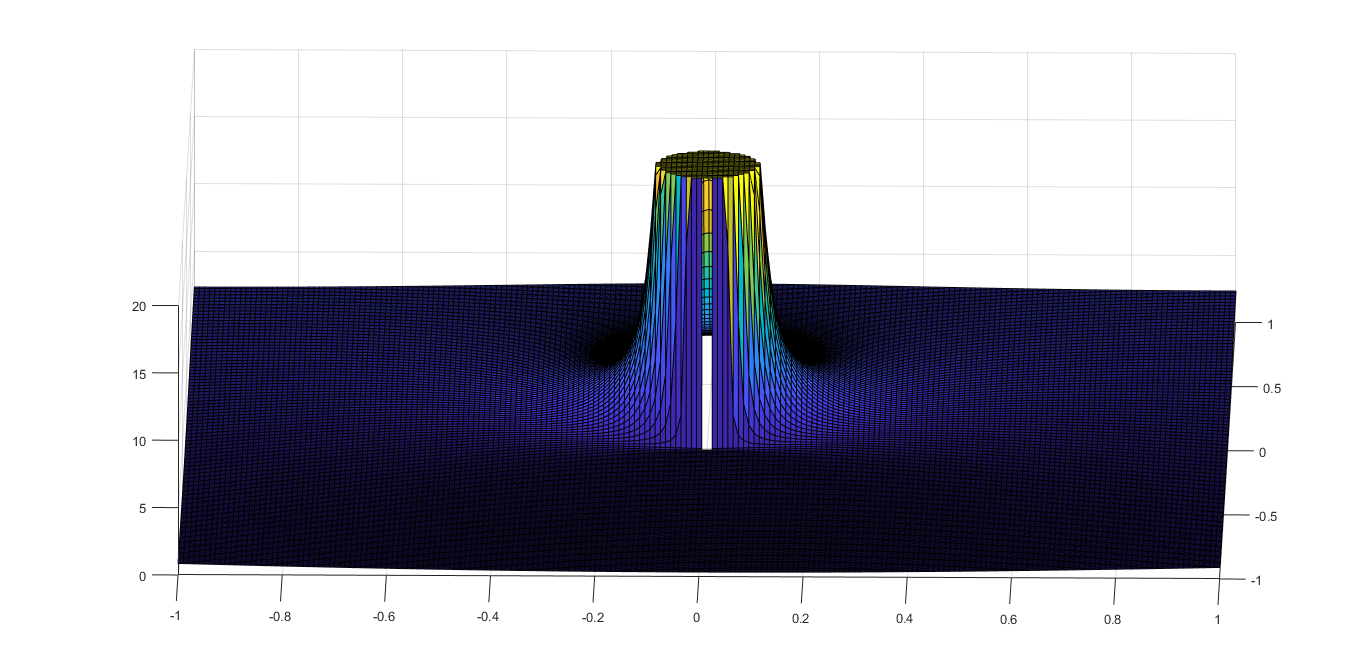
\includegraphics[scale = 0.3]{aout2017-7.png}
		\end{solfig}
		
		
		
	\end{enumerate}
	
\end{solution}


\section{}

Pour $m>0$, calculez l'intégrale suivante en utilisant le théorème des résidus:
$$\int_{0}^{\infty}{\frac{\cos(mx)}{1+x^2}dx}$$
Veillez à bien justifier toutes les étapes de calcul.\\
Note: les 5 lemmes de Jordan sont donnés.

\begin{solution}
	
	L'exercice est quasi identique à l'exercice 60 du syllabus écrit par Keunings. \\
	Calculons l'intégrale 
	$$\int_{C}{\frac{e^{imz}}{1+z^2}dz}$$
	avec $C$, le contour fermé en forme de demi-cercle illustré sur la figure ci-dessous.
	\begin{solfig}{c}{Contour d'intégration}
		\centering
		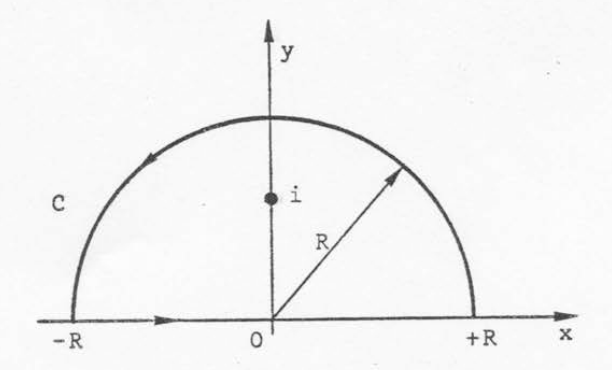
\includegraphics[scale = 0.4]{aout2017-6.png}
	\end{solfig}

	Ce contour entoure uniquement le pôle $z=i$. Le théorème des résidus s'énonce:\\
	Soit $f(z)$, une fonction holomorphe dans un domaine simplement connexe D sauf en un nombre fini de points $a_p$ qui sont des pôles ou des points singuliers essentiels de $f(z)$. Soit C une courbe fermée contenue dans D à l'intérieur de laquelle sont contenus tous les $a_p$. On a alors 
	$$\int_{C}f(z)dz=2\pi i \sum_{p=1}^{N}Res(a_p)$$
	où $Res(a_p)$ est le résidu de $f(z)$ relatif au point $a_p$.\\

	Ainsi, par ce théorème on a
	$$\int_{C}{\frac{e^{imz}}{1+x^2}dz}=2\pi i Res(i) $$
	$$\int_{-R}^R\frac{\cos(mx)}{1+z^2}dx+i\int_{-R}^R{\frac{\sin(mx)}{1+x^2}dx}+\int_{\Gamma}{\frac{e^{imz}}{1+z^2}dz}=2\pi i Res(i) $$
	avec $\Gamma$, la courbe $C$ dont on a enlevé le segment $[-R,R]$ sur l'axe réel. \\
	Le terme en sinus est nul car l'intégrant est impair et le domaine d'intégration est symétrique autour de l'origine.\\
	En faisant tendre $R$ à l'infini, le troisième terme est nul aussi par un des lemmes de Jordan:
	$$\lim_{R\rightarrow \infty}\int_{\Gamma}{\frac{e^{imz}}{1+x^2}dz}=\lim_{R\rightarrow \infty}\int_{\Gamma}{e^{imz}F(z)dz}$$
	avec $F(z)=1/(1+z^2)$. Le lemme de Jordan approprié précise que si $|F(z)|\leqslant M/R^k$ pour $z=Re^{i\theta}$, $M$ constante, $k>0$, alors 
	$$ \lim_{R\rightarrow \infty}\int_{\Gamma}{e^{imz}F(z)dz}=0 .$$
	On peut bien utiliser ce résultat car
	$$|F(z)|=\frac{1}{|1+R^2e^{2i\theta}|}<\frac{1}{|R^2||e^{2i\theta}|}=\frac{1}{R^2}=\frac{M}{R^k}$$
	avec $M=1$ et $k=2$.\\
	Finalement, 
	$$ \int_{-\infty}^\infty\frac{\cos(mx)}{1+x^2}dx=2\int_{0}^\infty\frac{\cos(mx)}{1+x^2}dx $$
	car l'intégrant est pair et le domaine d'intégration est symétrique autour de l'origine.\\
	On calcule ensuite le résidu:
	$$Res(i)= \lim_{z\rightarrow i}  \frac{e^{imz}}{i+z}=\frac{e^{-m}}{2i}$$
	 On obtient donc
	$$ 2\int_{0}^\infty\frac{\cos(mx)}{1+x^2}dx = 2\pi i \frac{e^{-m}}{2i}=\pi e^{-m} $$
	$$ \int_{0}^\infty\frac{\cos(mx)}{1+x^2}dx = \frac{\pi e^{-m}}{2}  $$
	
	
	
\end{solution}


\end{document}
